\documentclass[a4paper]{article}
\usepackage{fullpage}
\usepackage{graphicx}

\title{Life in Squares - Composing in Square Format}
\date{August 24, 2020}
\author{Jeremy Mudd}

\begin{document}
\maketitle


I’ve already shown you a few medium format cameras that make 6x6 square images, but I haven’t talked much about the art of composing in square format. You may ask - Isn’t it the same thing as composing in 4x5 or more modern 2x3 format? Don’t the same rules apply?  

The simple answer is “yes and no”.  

Before I go too deep into this subject though, I want to say up front that “rules” in photography are made to be just general guidelines. It’s good to know them, so that later in your photographic journey you know when you can break them.    

The first thing you will notice when you pick up a square-format camera is that you no longer need to worry about turning the camera on its side for portrait, or keeping horizontal for landscape. It’s all the same. That may sound obvious, but I remember the first time I shot with one I caught myself turning the camera on its side, and laughing at myself when I realized what I was doing. After spending some time shooting in this manner, I came to realize this one simple fact is very freeing. 

You might think that shooing in a square format is restrictive. And to a point, that’s true. Sometimes, it’s the restrictions that cause us to be most creative. It’s this restriction that enabled me to start thinking about my shots as they related to the format.

\section*{MOVEMENT THROUGH THE FRAME}
When you compose and shoot in landscape orientation, generally the shape of the image moves the viewer’s eyes side to side. When you compose and shoot in portrait orientation, the eye movement is typically up and down. A square image typically causes the viewer to move their eyes around the frame inside in a circular motion. 

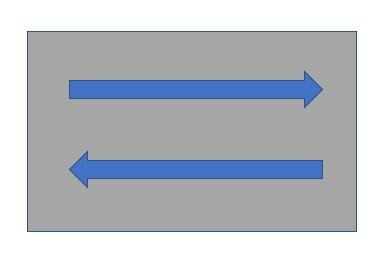
\includegraphics[width=50mm]{img/Horizontal.jpeg}
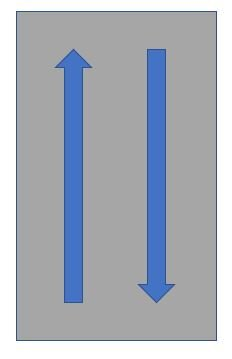
\includegraphics[width=50mm]{img/Vertical.jpeg}
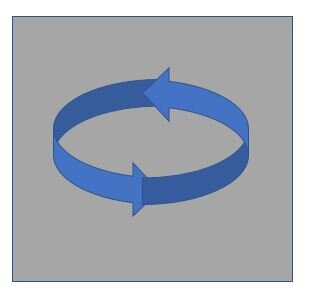
\includegraphics[width=50mm]{img/Square.jpeg}

These three shots below of the same subject illustrate this point. 
\begin{figure}[ht!]
    \centering
    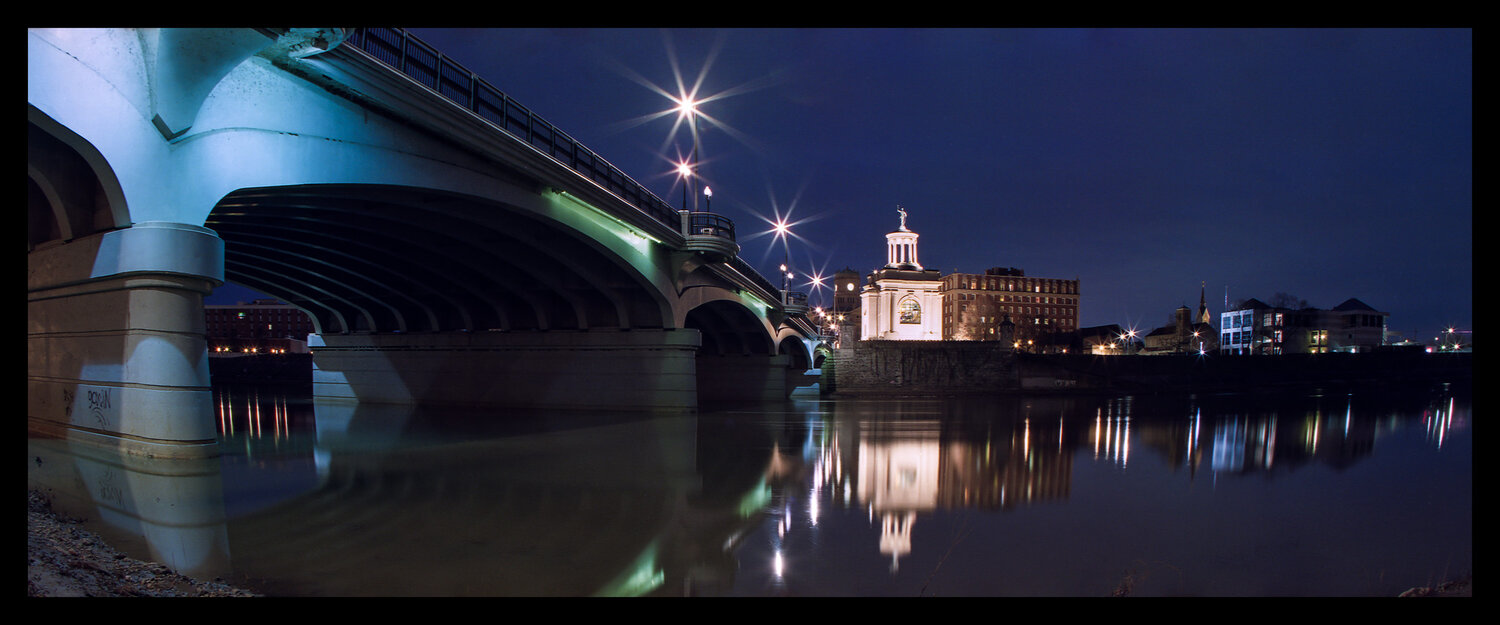
\includegraphics[width=150mm]{img/49646000797_6f1991f098_k.jpeg}
    \caption{Hamilton, Ohio - shot on a double-wide section of 35mm film (70x24mm) for a wide landscape orientation. The viewers eyes will tend to move side to side in the frame, aided by the leading line of the bridge to the left.}
\end{figure}

\begin{figure}[ht!]
    \centering
    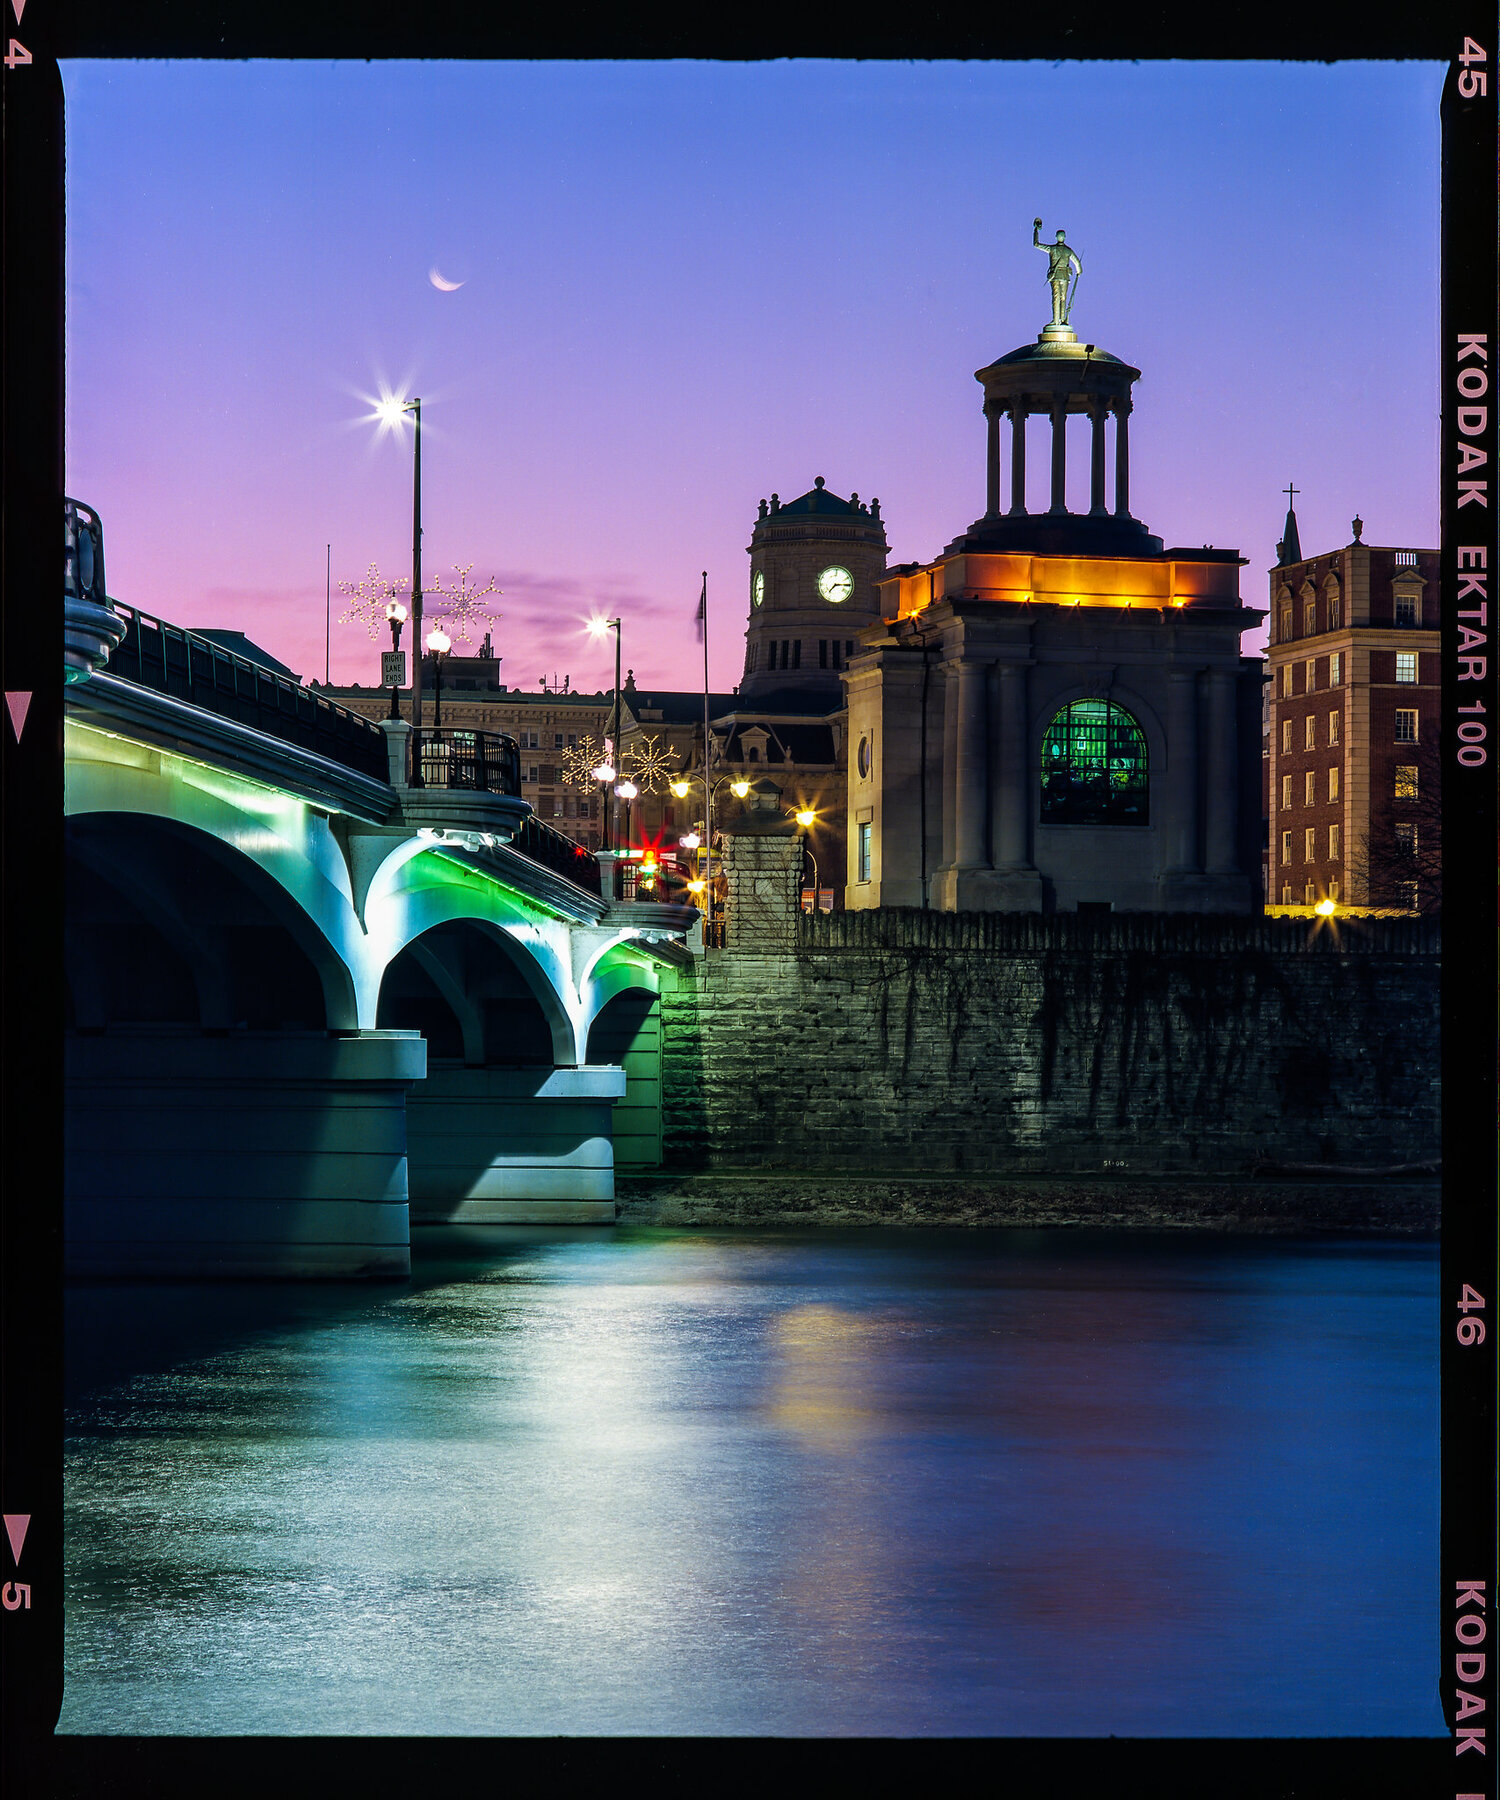
\includegraphics[width=90mm]{img/39114574851_e9da9d4720_k.jpeg}
    \caption{Hamilton, Ohio - shot on a Mamiya RB67 in portrait mode for a 6cm x 7cm vertical image. Again the bridge affects the eye movement thru the frame, but now its more vertical due to the shape of the frame.}
\end{figure}

\begin{figure}[ht!]
    \centering
    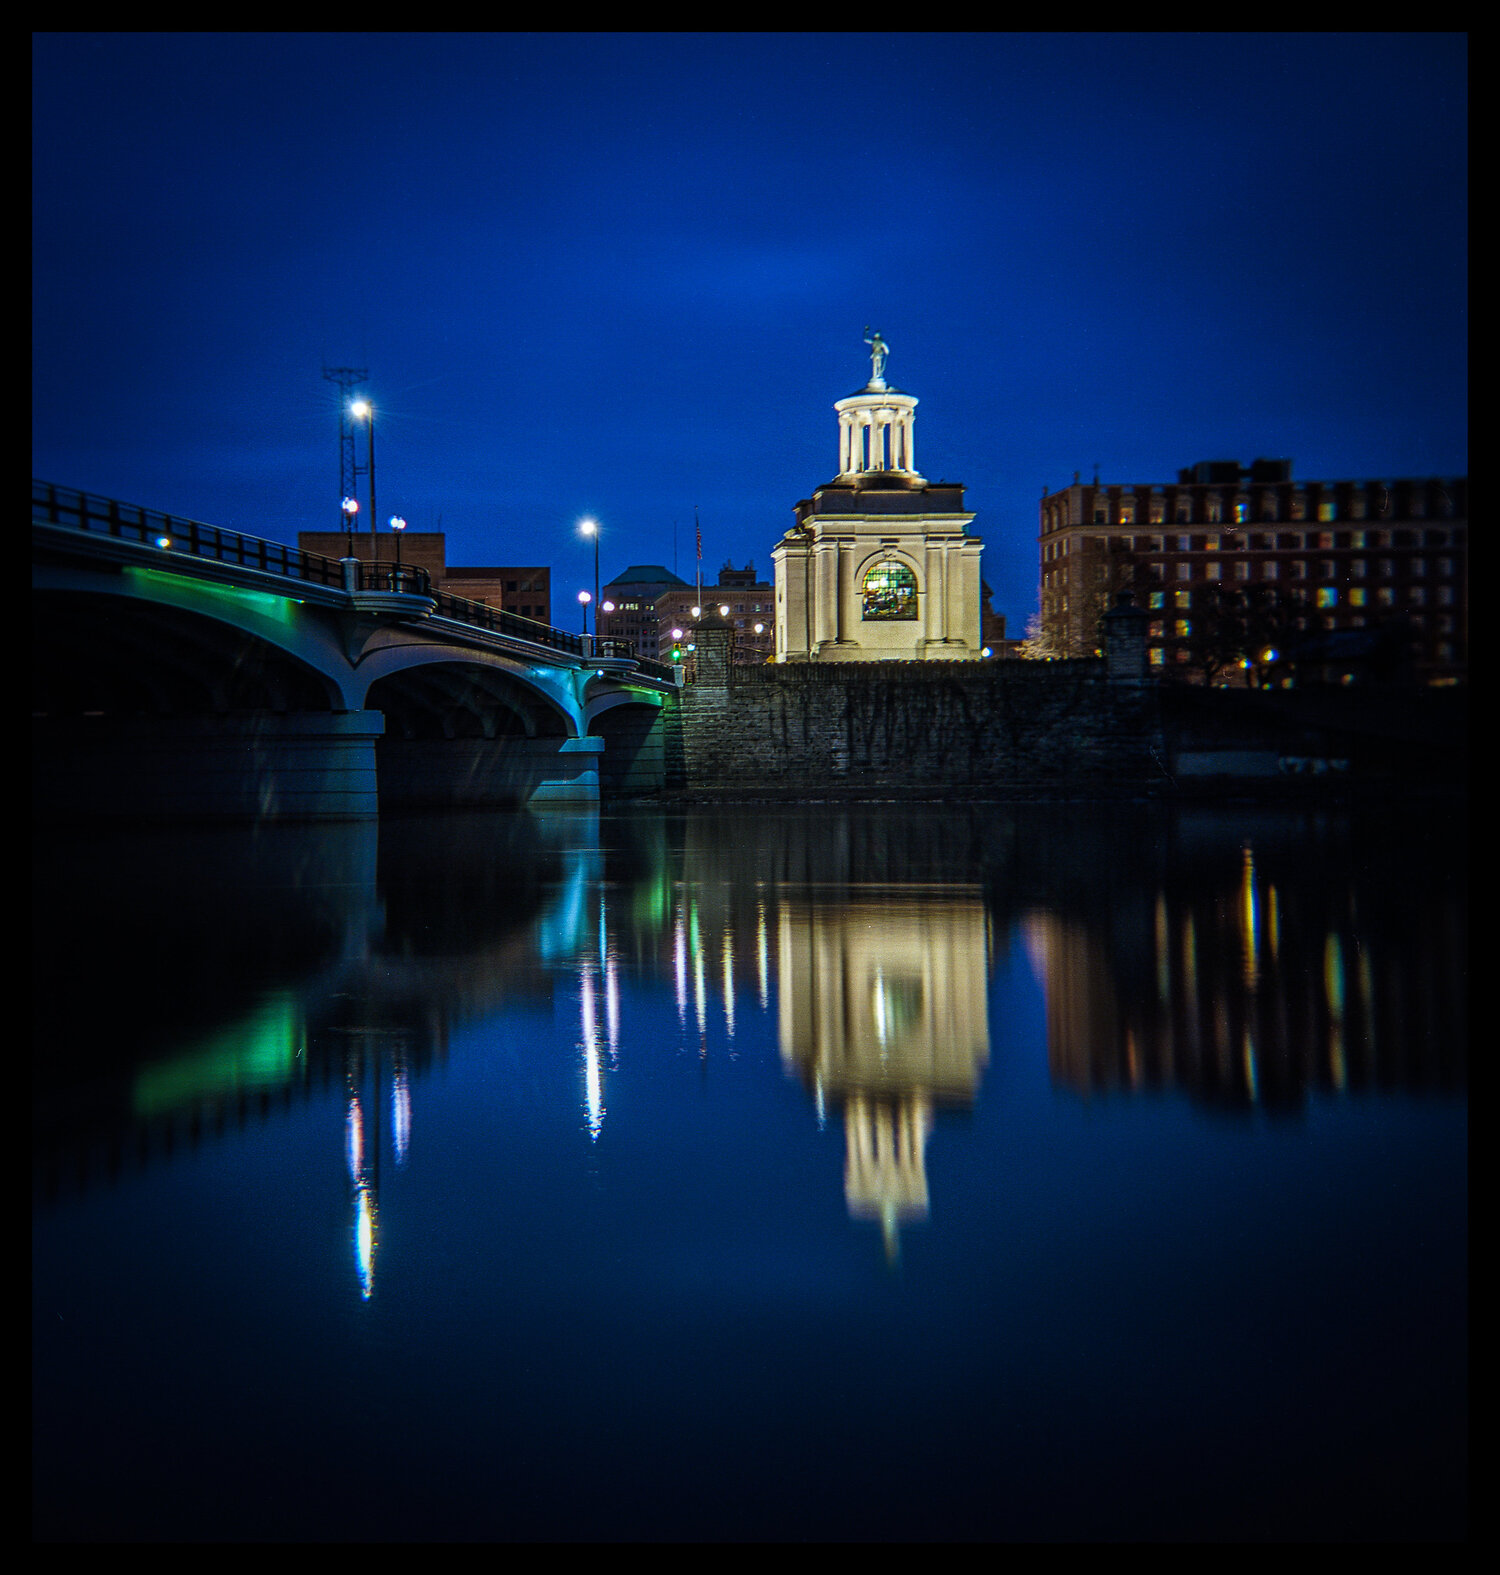
\includegraphics[width=90mm]{img/image-asset.jpeg}
    \caption{Hamilton, Ohio - shot on a Holga 120N square format camera. Due to the square format the eyes tend to move around in the middle of the frame and explore what’s there. Also, apparently I like to photograph in Hamilton quite a bit, eh?}
\end{figure}

\section*{CENTRAL COMPOSITION}
Given the tendancy for circular movement in a square frame, putting your subject in the very middle of the square frame often makes the most sense. This totally flies in the face of the Rule of Thirds, and that’s OK.  Another benefit to putting your subject in the middle is, especially in the case of Holga’s, that the middle portion is the sharpest part of the lens. Also, a lot of older medium format glass also has a really nice bokeh effect, and having that swirling around the subject in the middle further enhancing the nice medium format depth of field “look”.  

\begin{figure}[ht!]
    \centering
    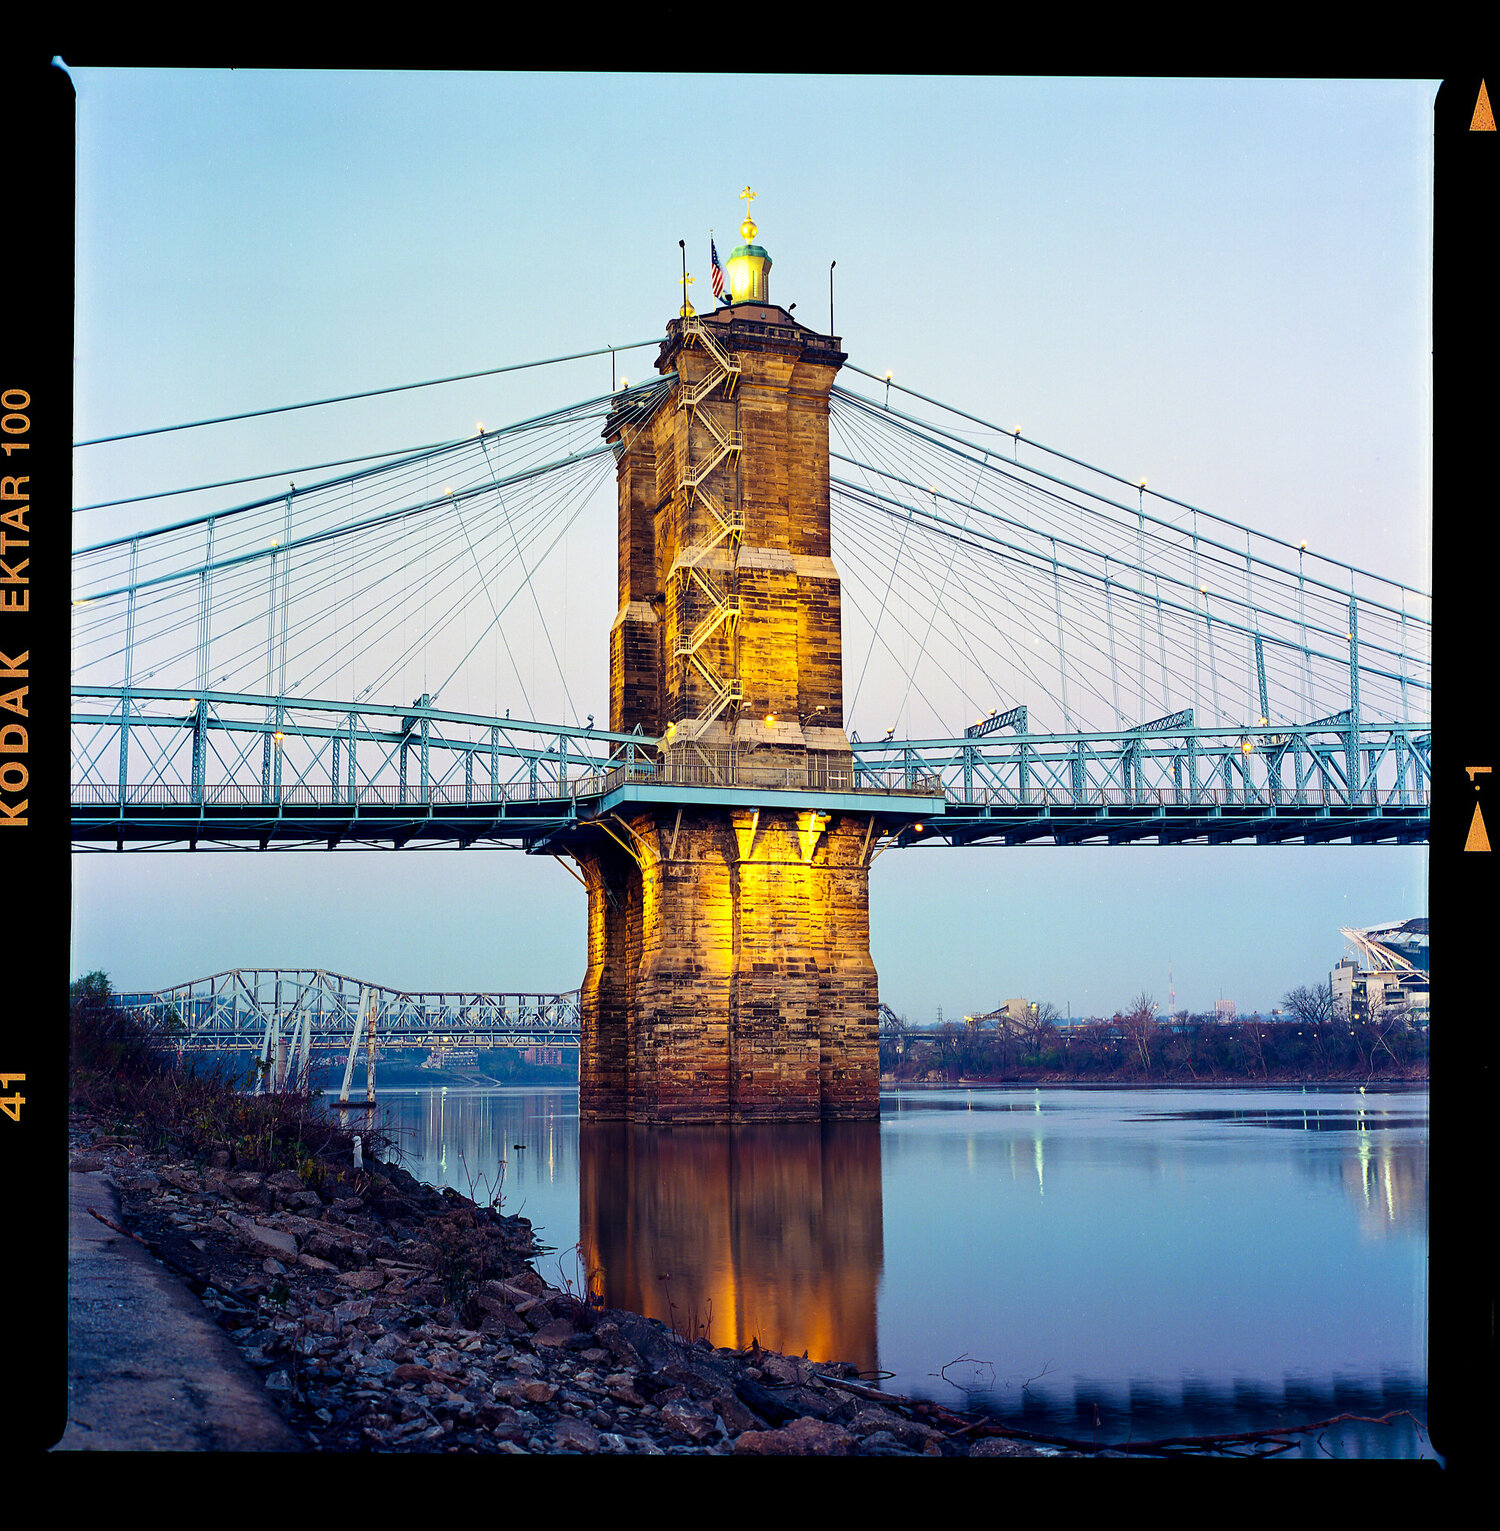
\includegraphics[width=90mm]{img/24999764268_54169a5804_k.jpeg}
    \caption{Roebling Bridge in Blue Hour - Bronica S2A on Kodak Ektar film. The bridge upright is in the center, and the road also intersects that upright in the center.}
\end{figure}

\begin{figure}[ht!]
    \centering
    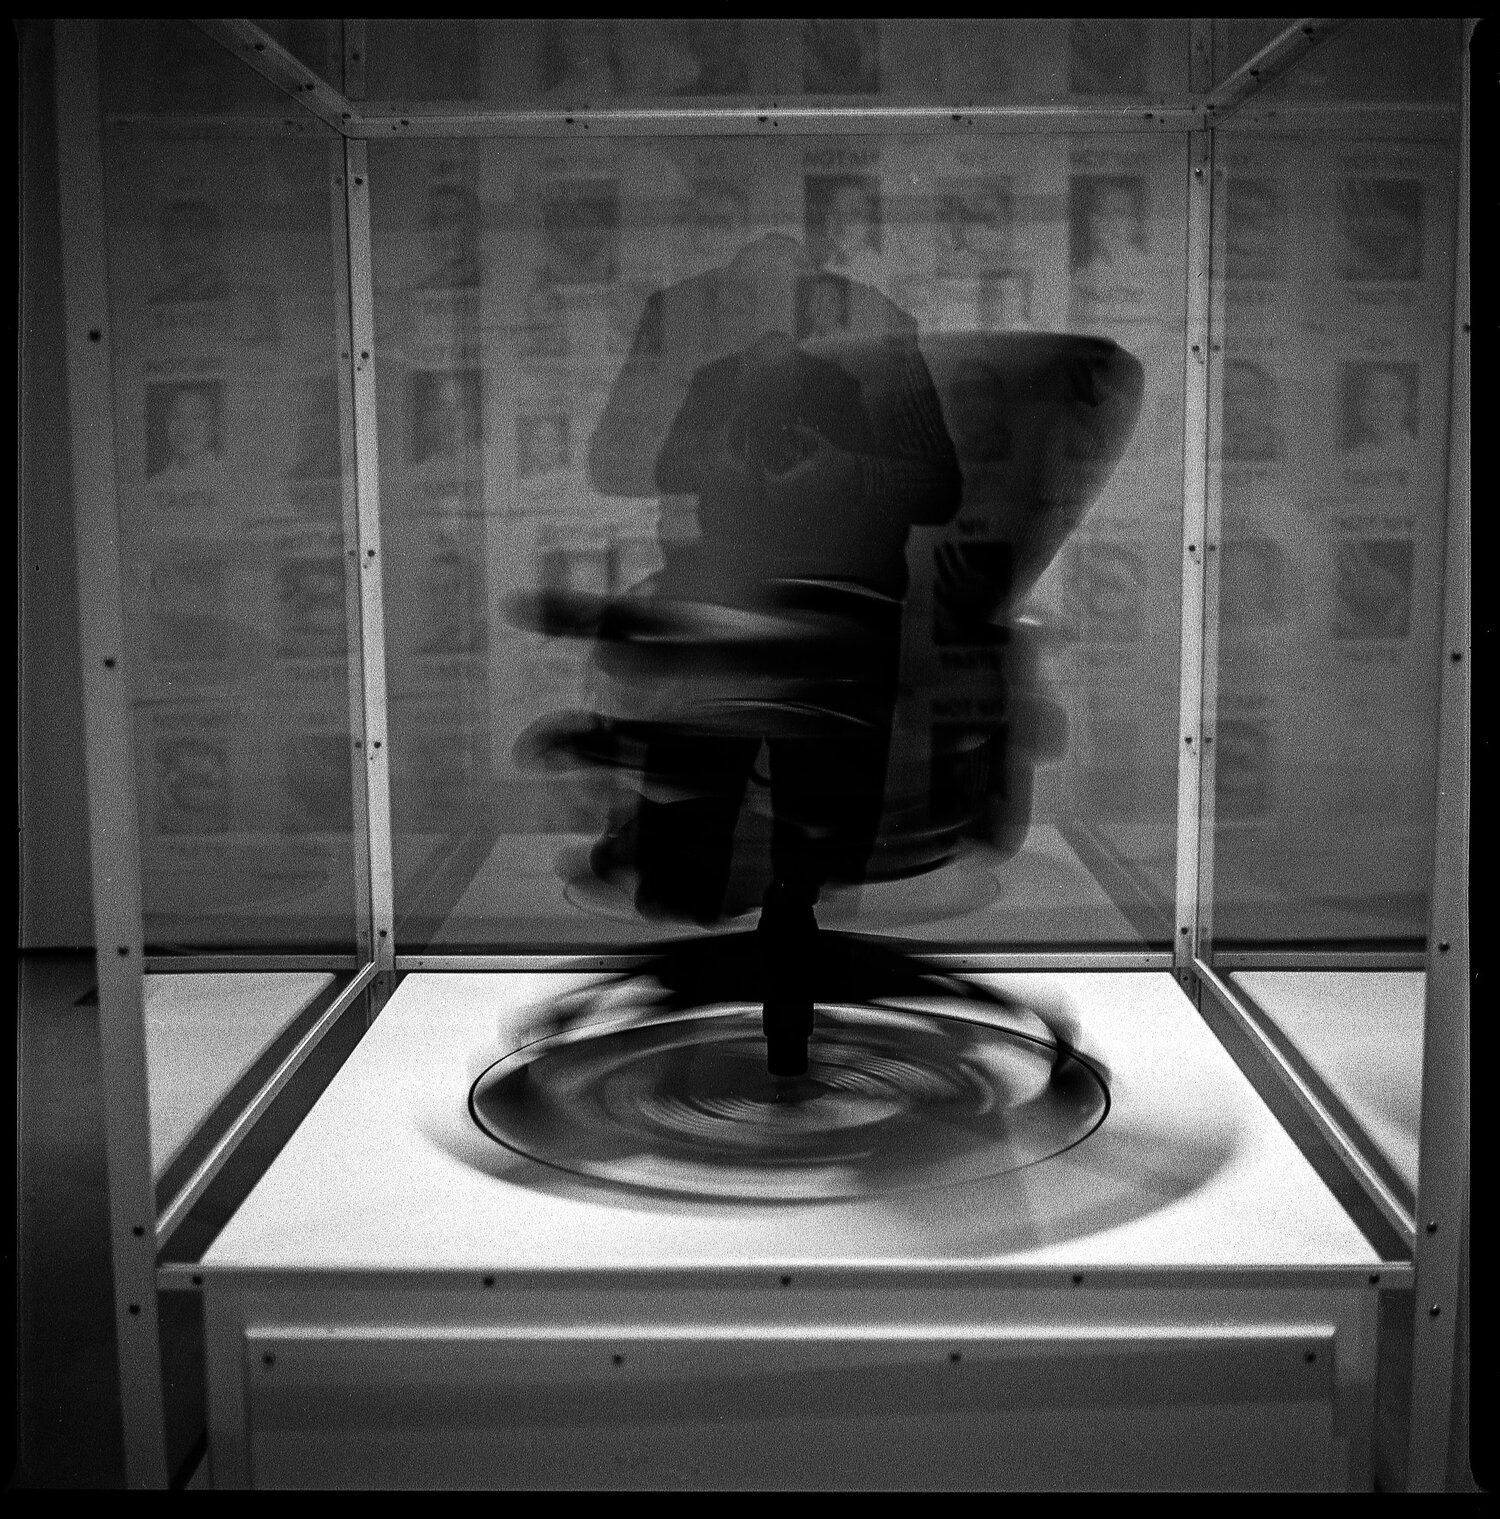
\includegraphics[width=90mm]{img/38908023902_4baf06c19e_k.jpeg}
    \caption{Spinning Chair Selfie - Bronica S2A. The spinning chair has a great sense of motion due to the blur from the slow shutter speed, and being in the center allows the eyes to move around it and be part of the motion. The double reflection of me looking down into the Bronica viewfinder was a bonus.}
\end{figure}

\begin{figure}[ht!]
    \centering
    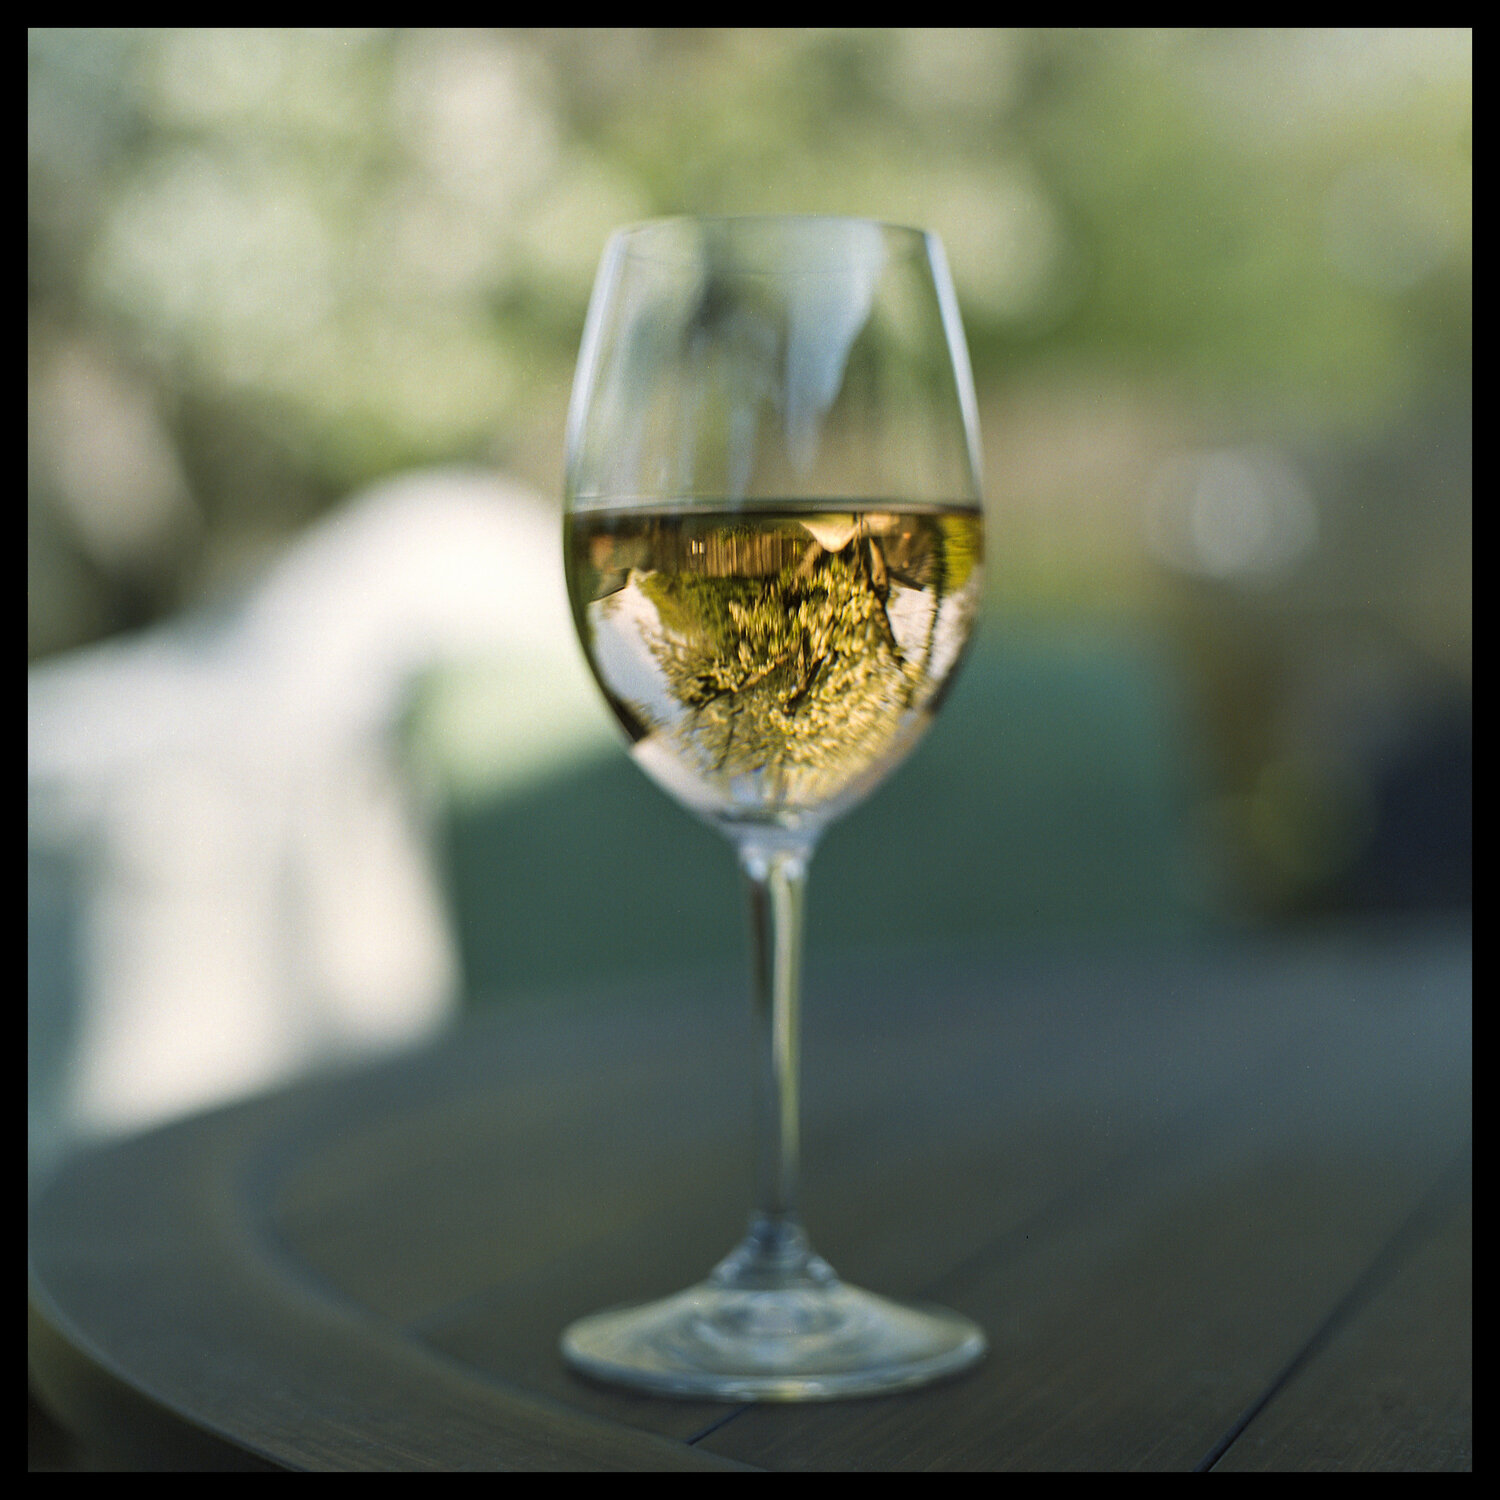
\includegraphics[width=90mm]{img/49839226537_a983ab355f_k.jpeg}
    \caption{Chardonnay and Crabapple Tree - Kowa Six camera with Portra NC film. Putting the subject in the middle makes for a nice composition in square format, plus takes advantage of the sharp medium format lens and nice background bokeh.}
\end{figure}

\section*{SIMPLICITY}
Shooting in square format lends itself naturally to a more simple approach. I think this is because there isn’t a great deal of extra room at the top or sides, so trying to simplify it becomes necessary.  

\begin{figure}[ht!]
    \centering
    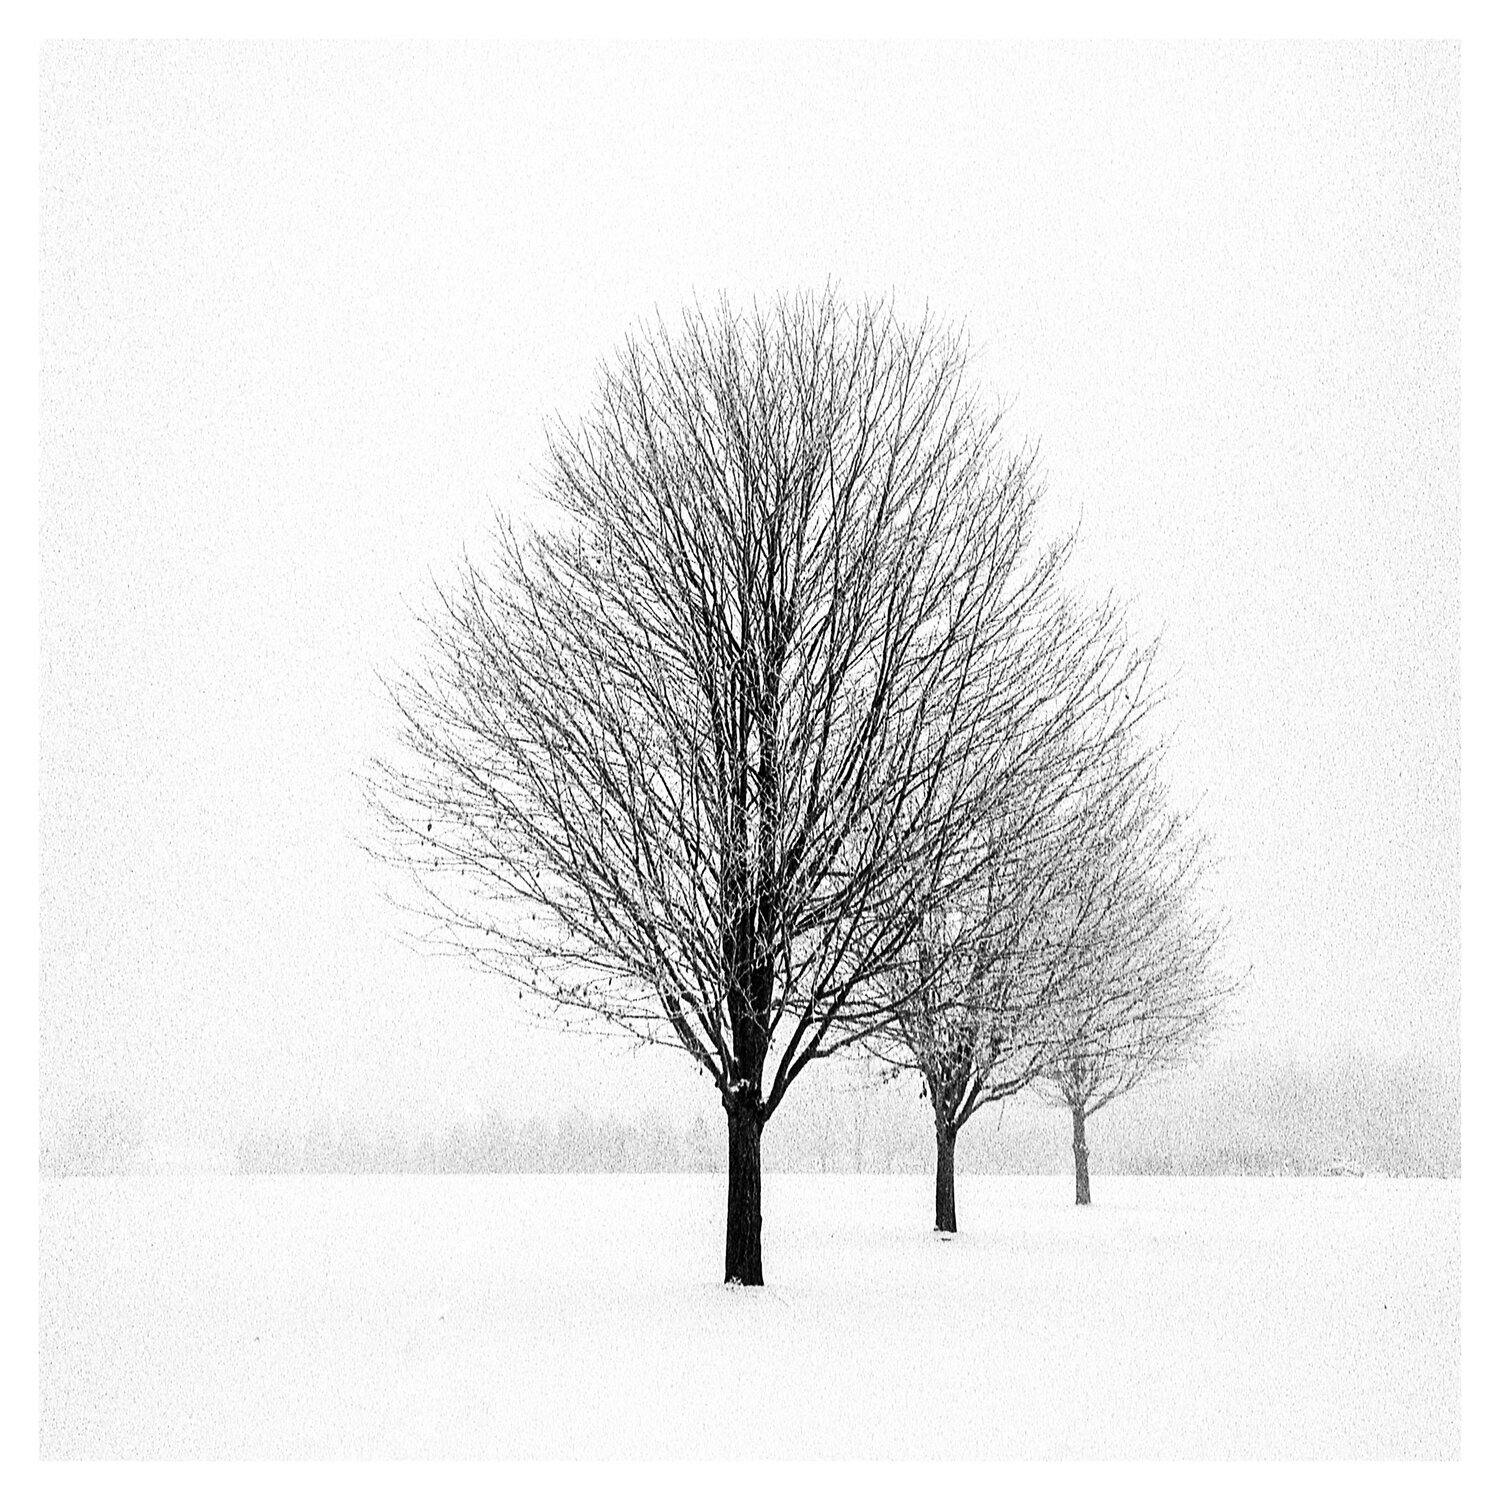
\includegraphics[width=90mm]{img/46248701704_c6af502fba_k.jpeg}
    \caption{Snow and Freezing Fog - National Museum of the USAF. Shot with a Hasselblad 500c. The snow and fog did a great job of simplifying the scene for me. I shot this several different ways that day, but this simple composition was my favorite.}
\end{figure}

\begin{figure}[ht!]
    \centering
    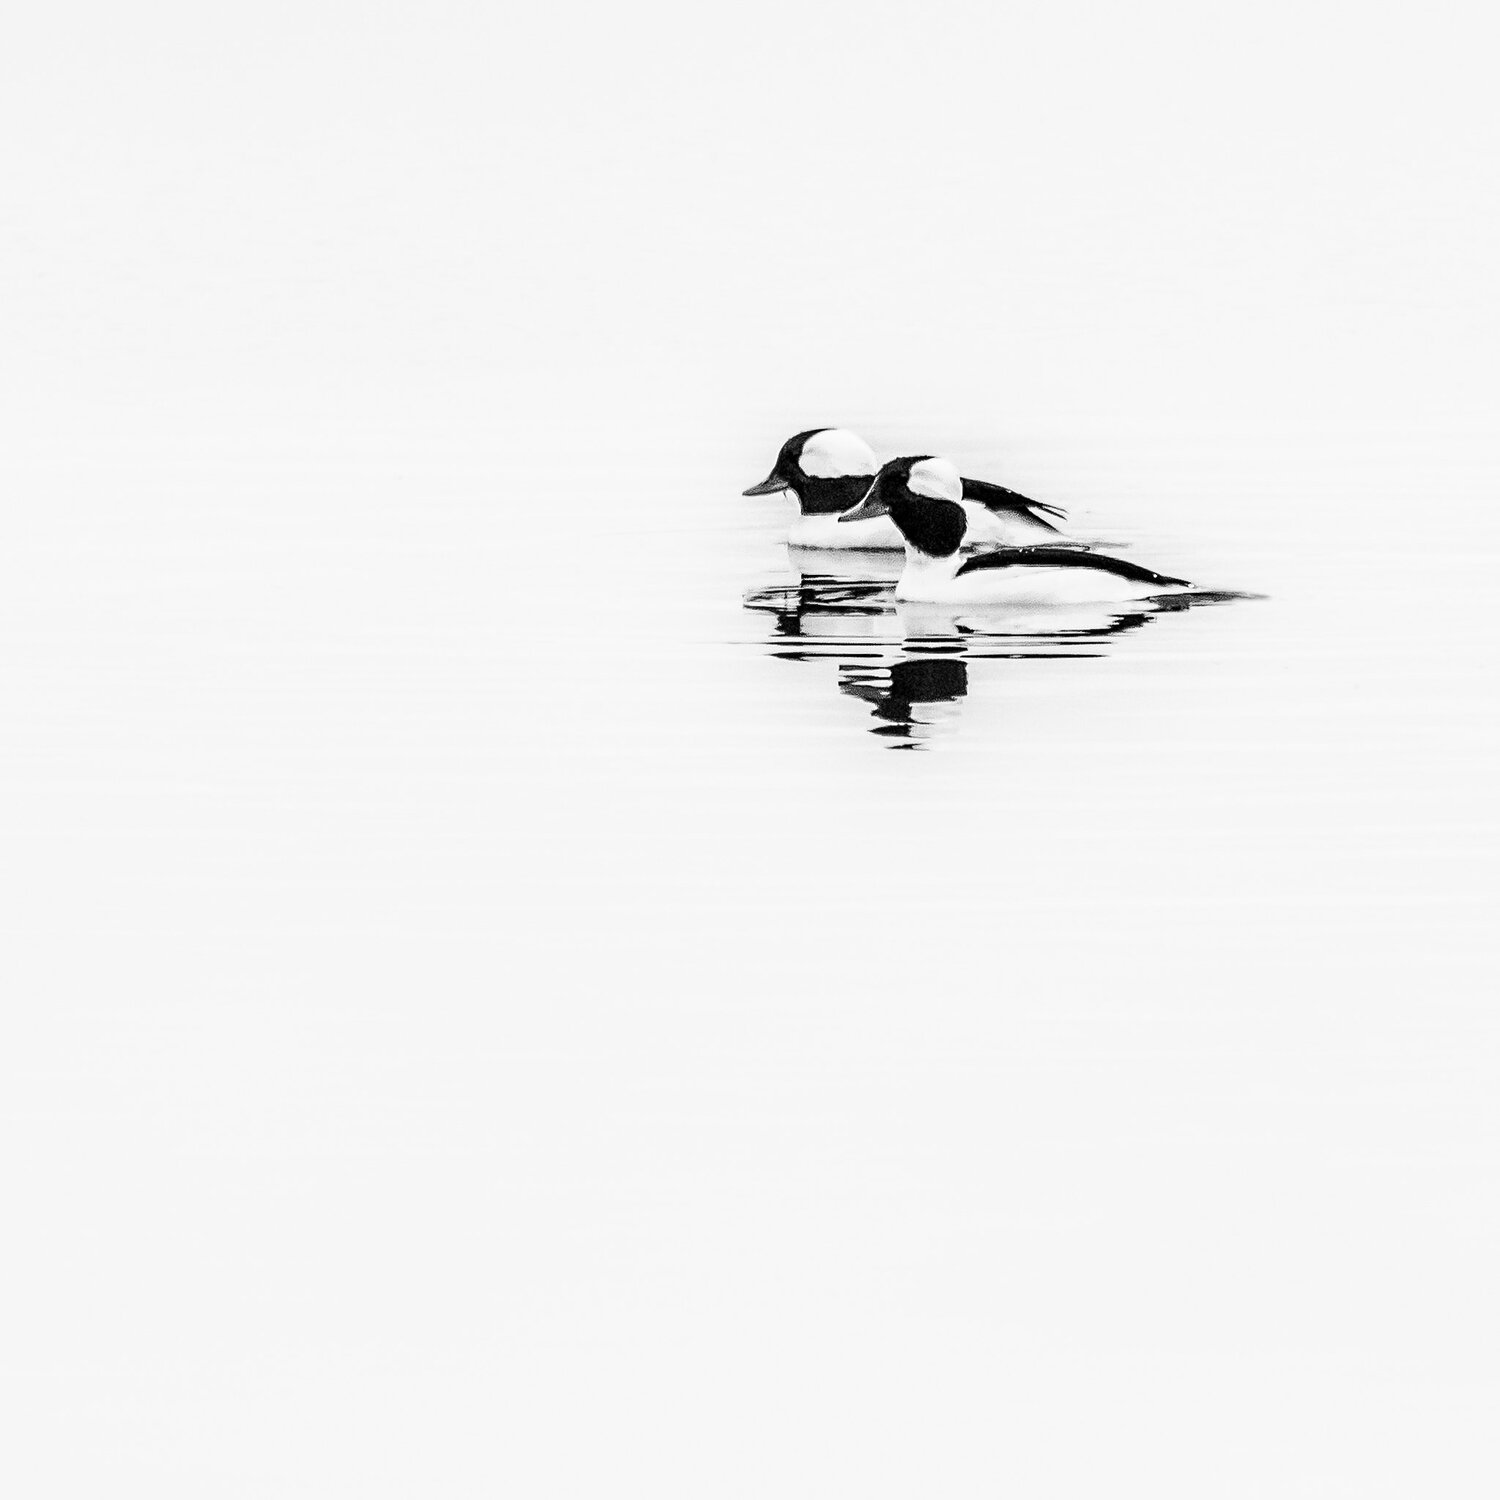
\includegraphics[width=90mm]{img/45972195685_ae6d923431_k.jpeg}
    \caption{Two Buffleheads - Hasselblad 500c on Tri-X 400 film. So I fired off two images before the birds took off. The first was them dead center, the second was this one. This is probably one of the most simple images I’ve shot in a long while. The birds are also, as a bonus, placed right on the intersection of two outer lines for the Rule of Thirds.}
\end{figure}

To me, there is no better master at simplicity than Michael Kenna. Some of his work from Japan is just incredible.  See some of Kenna’s work here.

\section*{SYMMETRY} 
Once again, I’m talking about breaking that ever-popular Rule of Thirds here. Symmetry is great for making a strong visual that incorporates the entire weight of the frame. This really shines in the square format, but be careful about not over-doing this one. You don’t want so much busy symmetry that your image starts to look like a child’s kaleidoscope.  

\begin{figure}[ht!]
    \centering
    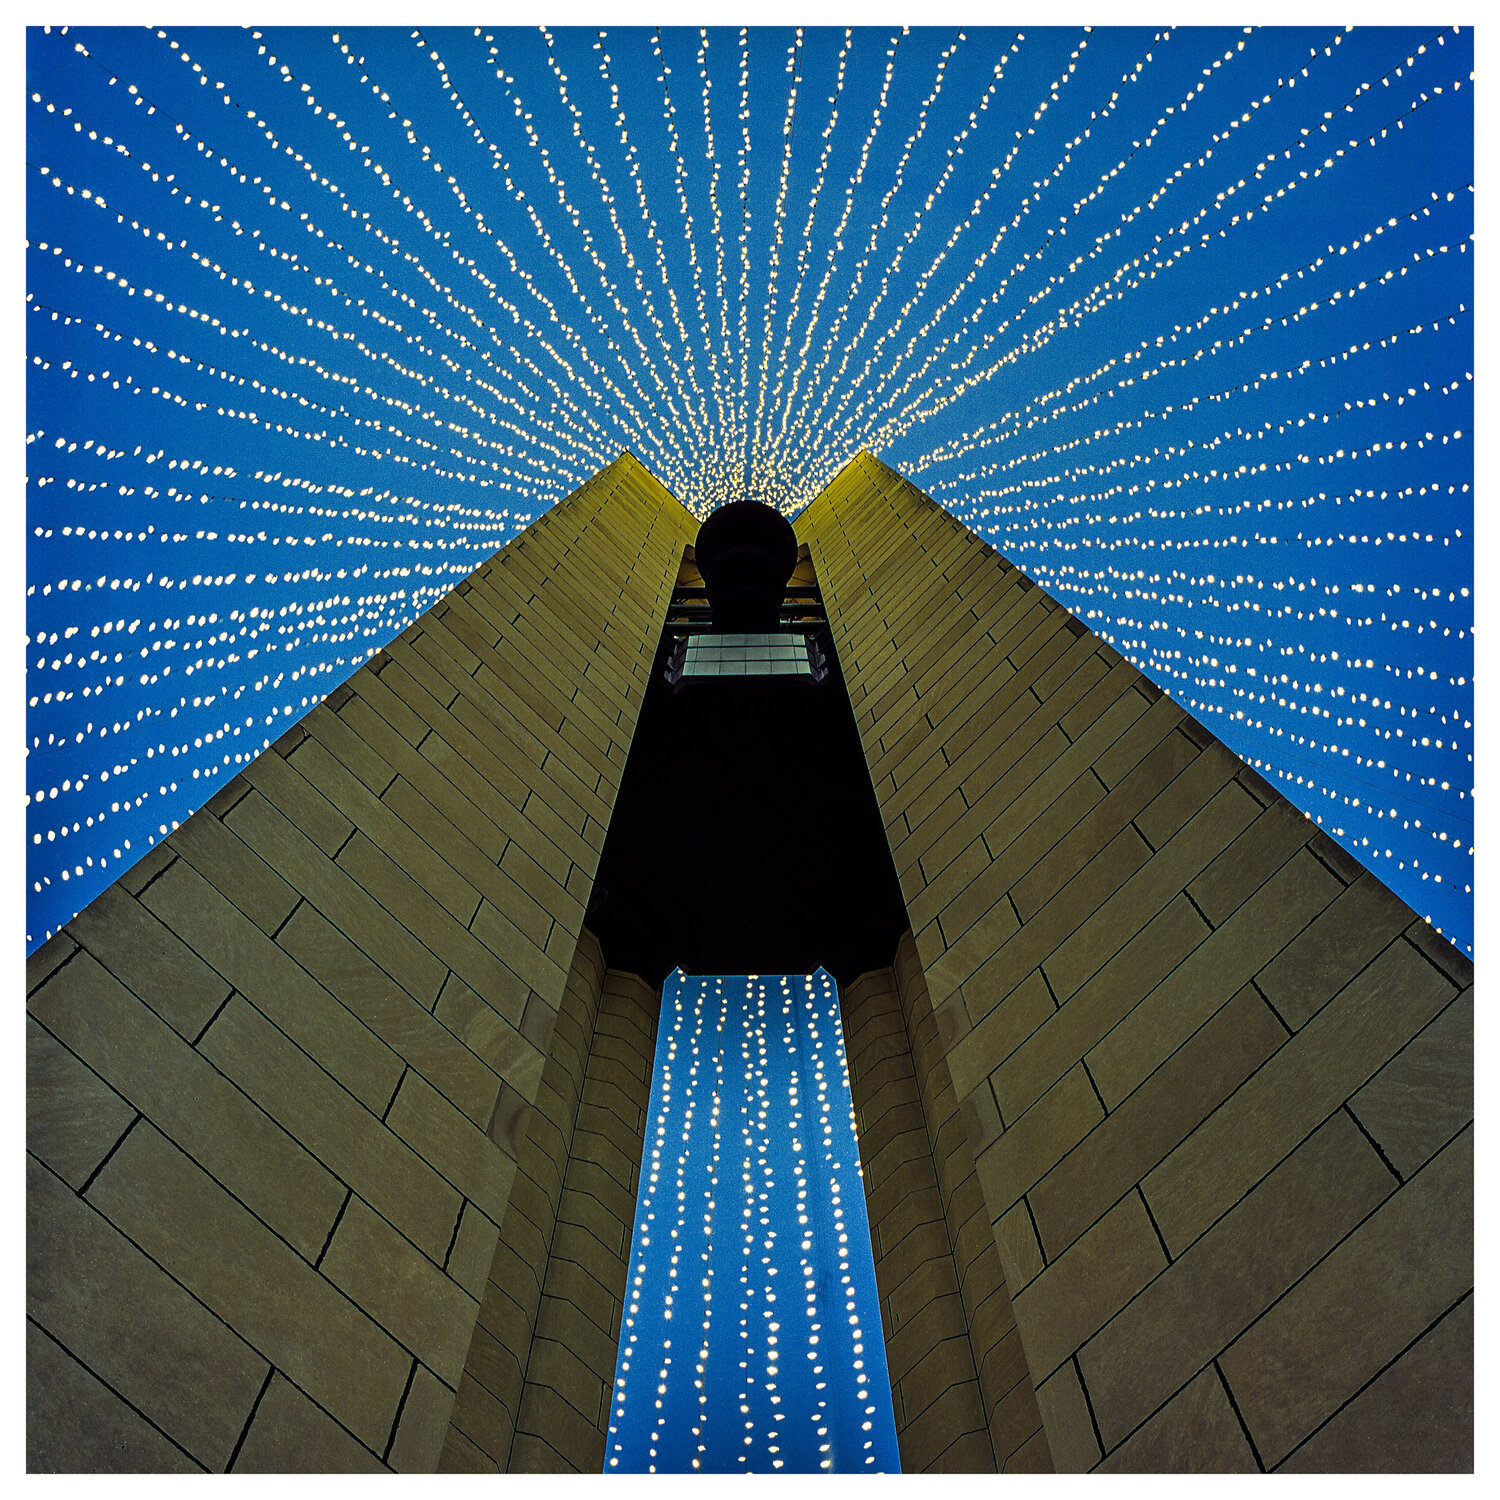
\includegraphics[width=90mm]{img/49224084658_765dbc83a6_k.jpeg}
    \caption{Carillon Park bell tower at Christmas- Hasselblad 500c on Kodak Ektar film during the blue hour. I shot a few other compositions of this where I put the tower off-center - but they just didn’t work for me.}
\end{figure}

\begin{figure}[ht!]
    \centering
    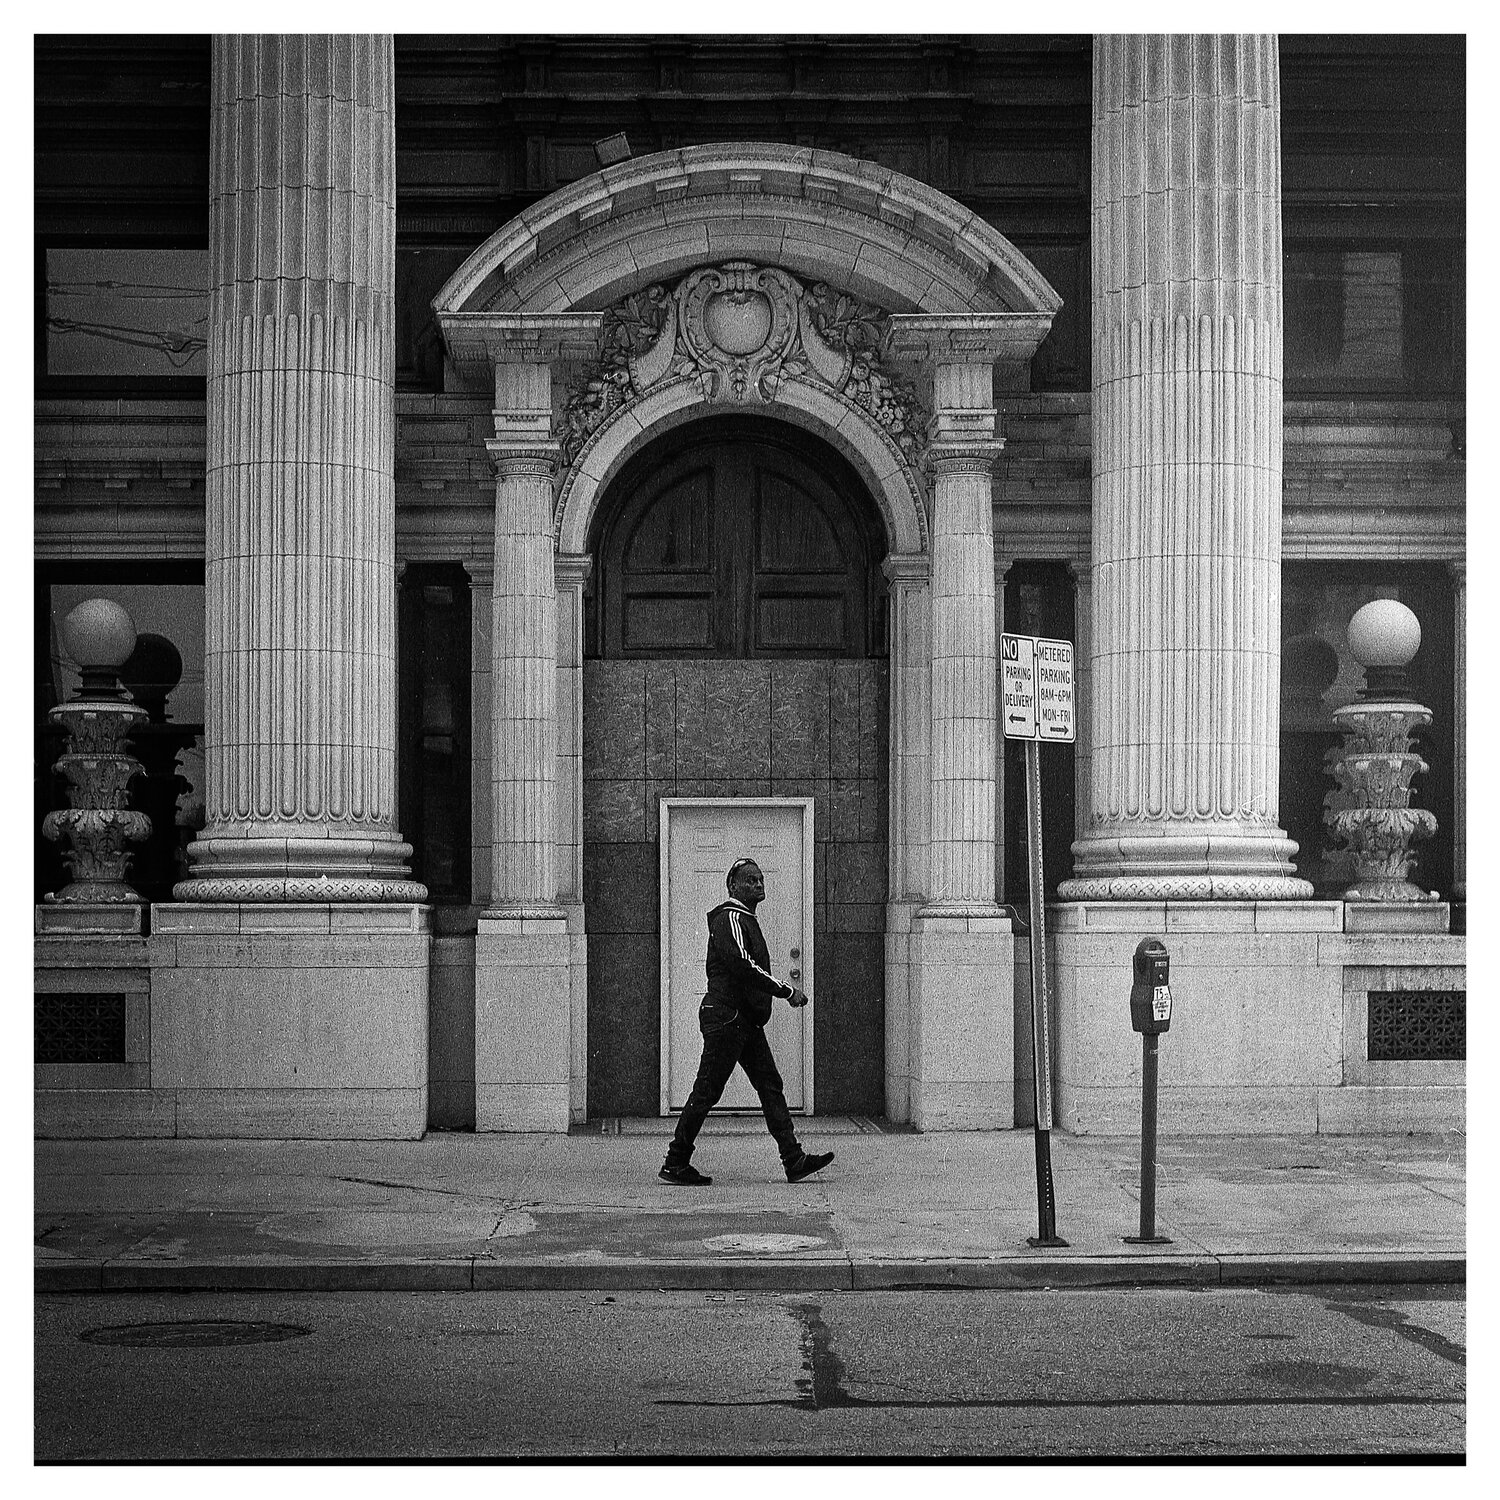
\includegraphics[width=90mm]{img/33898121918_1c5aff9da0_k.jpeg}
    \caption{This the old Dayton Daily News building in downtown Dayton, Ohio. Shot on my Yashica-Mat TLR. While I was lining up the shot I saw out of the corner of my left eye this gentleman approaching so I paused for a moment for him to be dead center.}
\end{figure}

\begin{figure}[ht!]
    \centering
    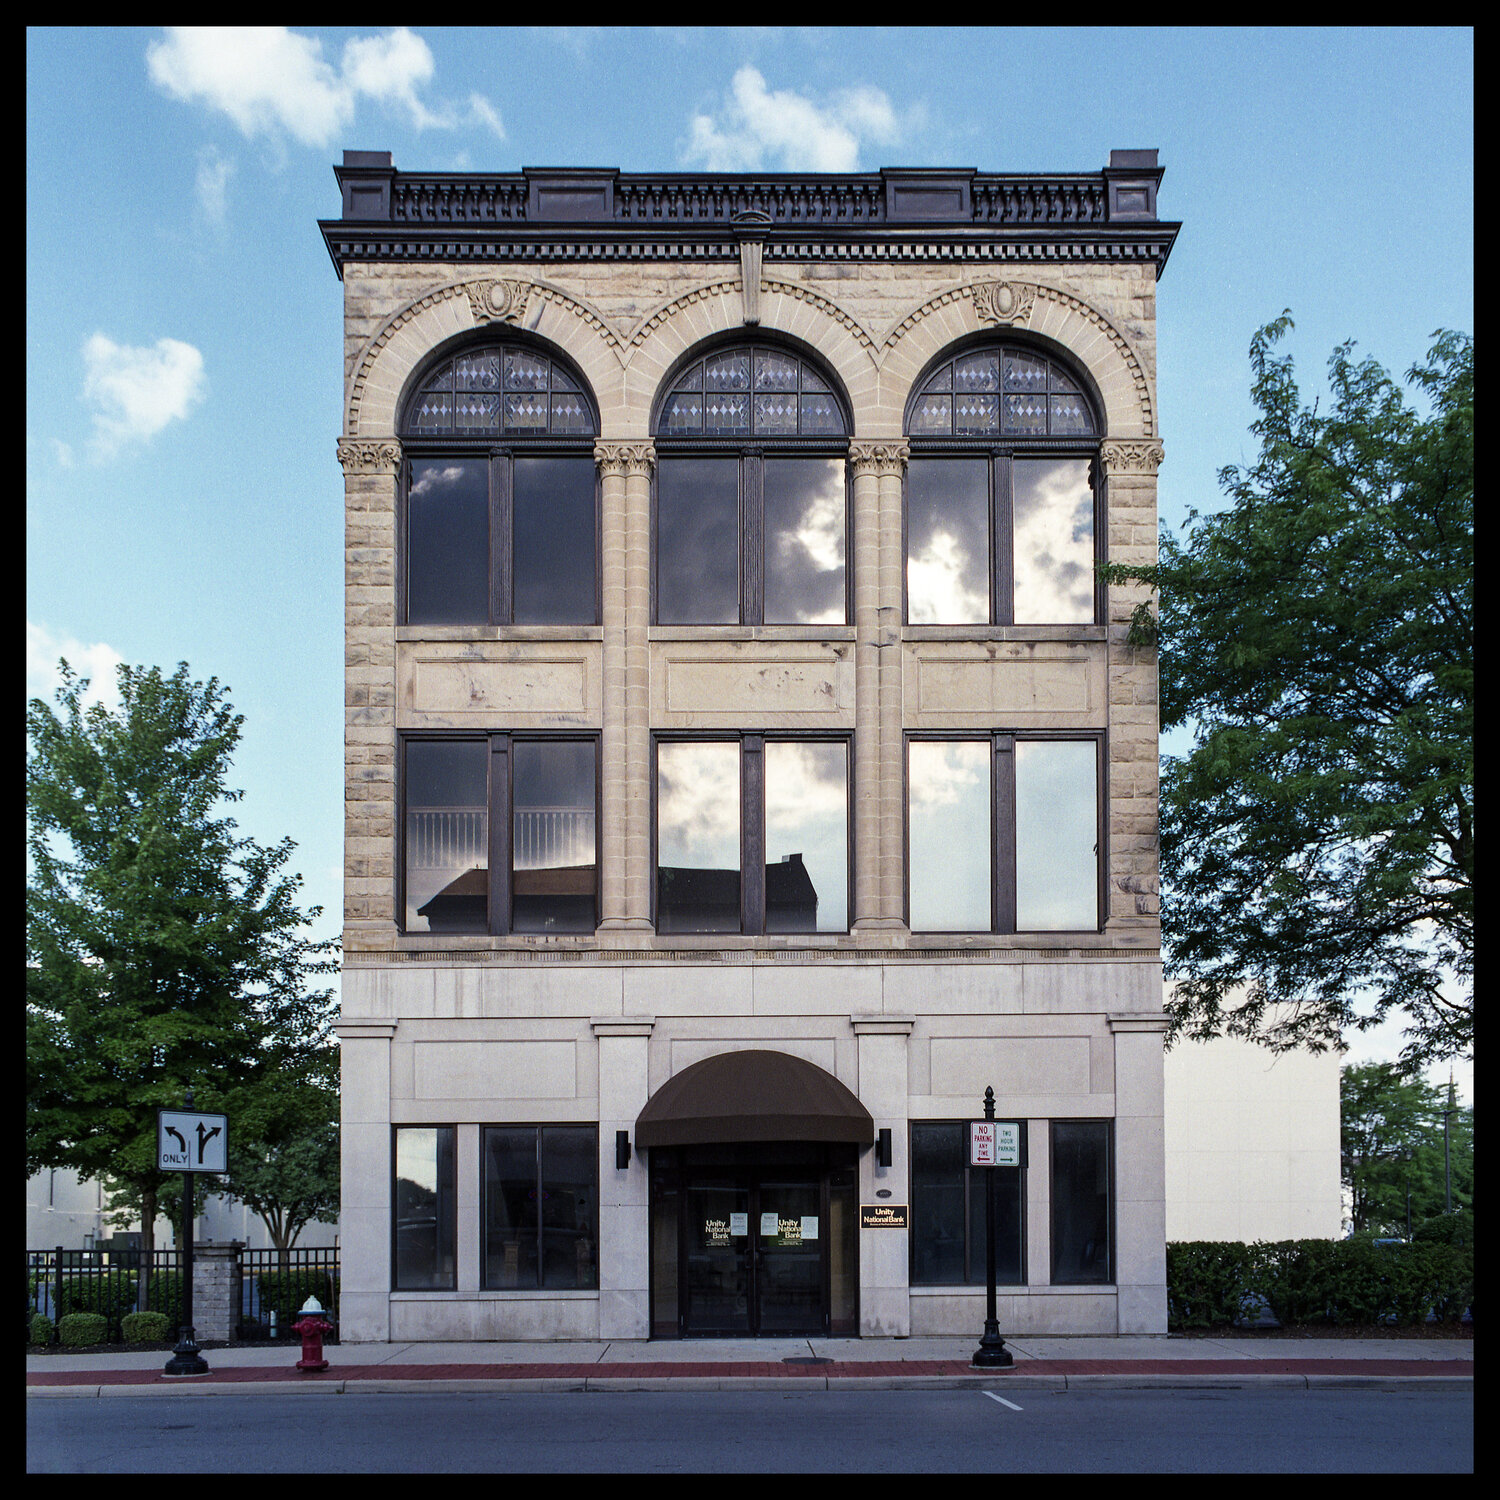
\includegraphics[width=90mm]{img/50177784312_77ddedaa9c_k.jpeg}
    \caption{Old building in downtown Piqua, Ohio. Shot on my Kowa Six on Fuji Pro 400H film. The symmetry of the building works well here, accented by the reflected sky in the windows.}
\end{figure}

\section*{LEADING LINES}
OK, this one is fairly common for ALL shapes of images, but don’t forget about it with square format. Just because there isn’t a wide or tall frame doesn’t mean leading lines don’t have a place. If done well it can be a very dramatic effect in a square frame.  

\begin{figure}[ht!]
    \centering
    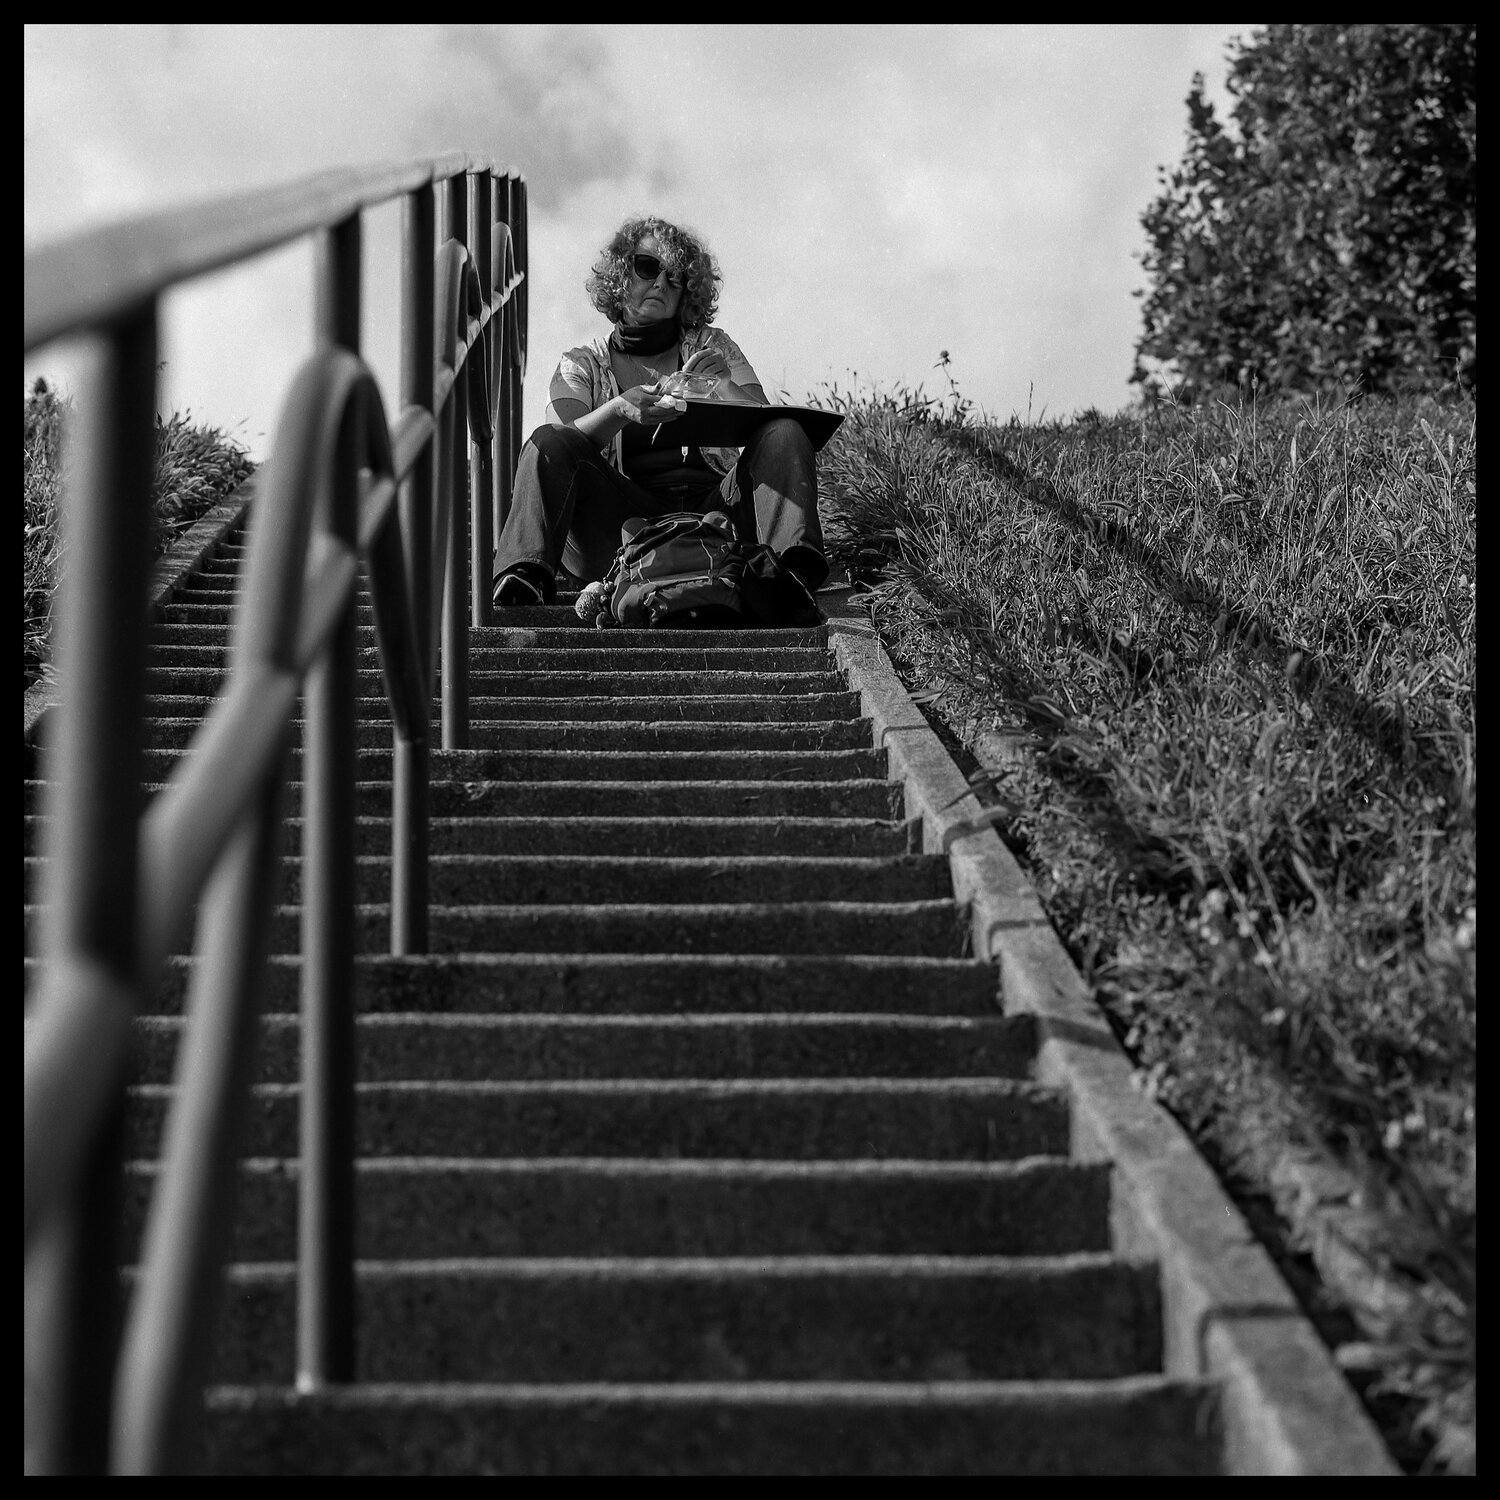
\includegraphics[width=90mm]{img/50234103591_81c88c5aec_k.jpeg}
    \caption{Renee doing watercolor down near McPherson in Dayton, Ohio. Kowa Six on Tri-X 400 film. She looks angry in this pic - not certain if its directed at me for taking the image or the two women who just walked by on the stairs with no masks on. Obvious use of the stairs and railing as leading lines directing attention upwards toward the subject.}
\end{figure}

\begin{figure}[ht!]
    \centering
    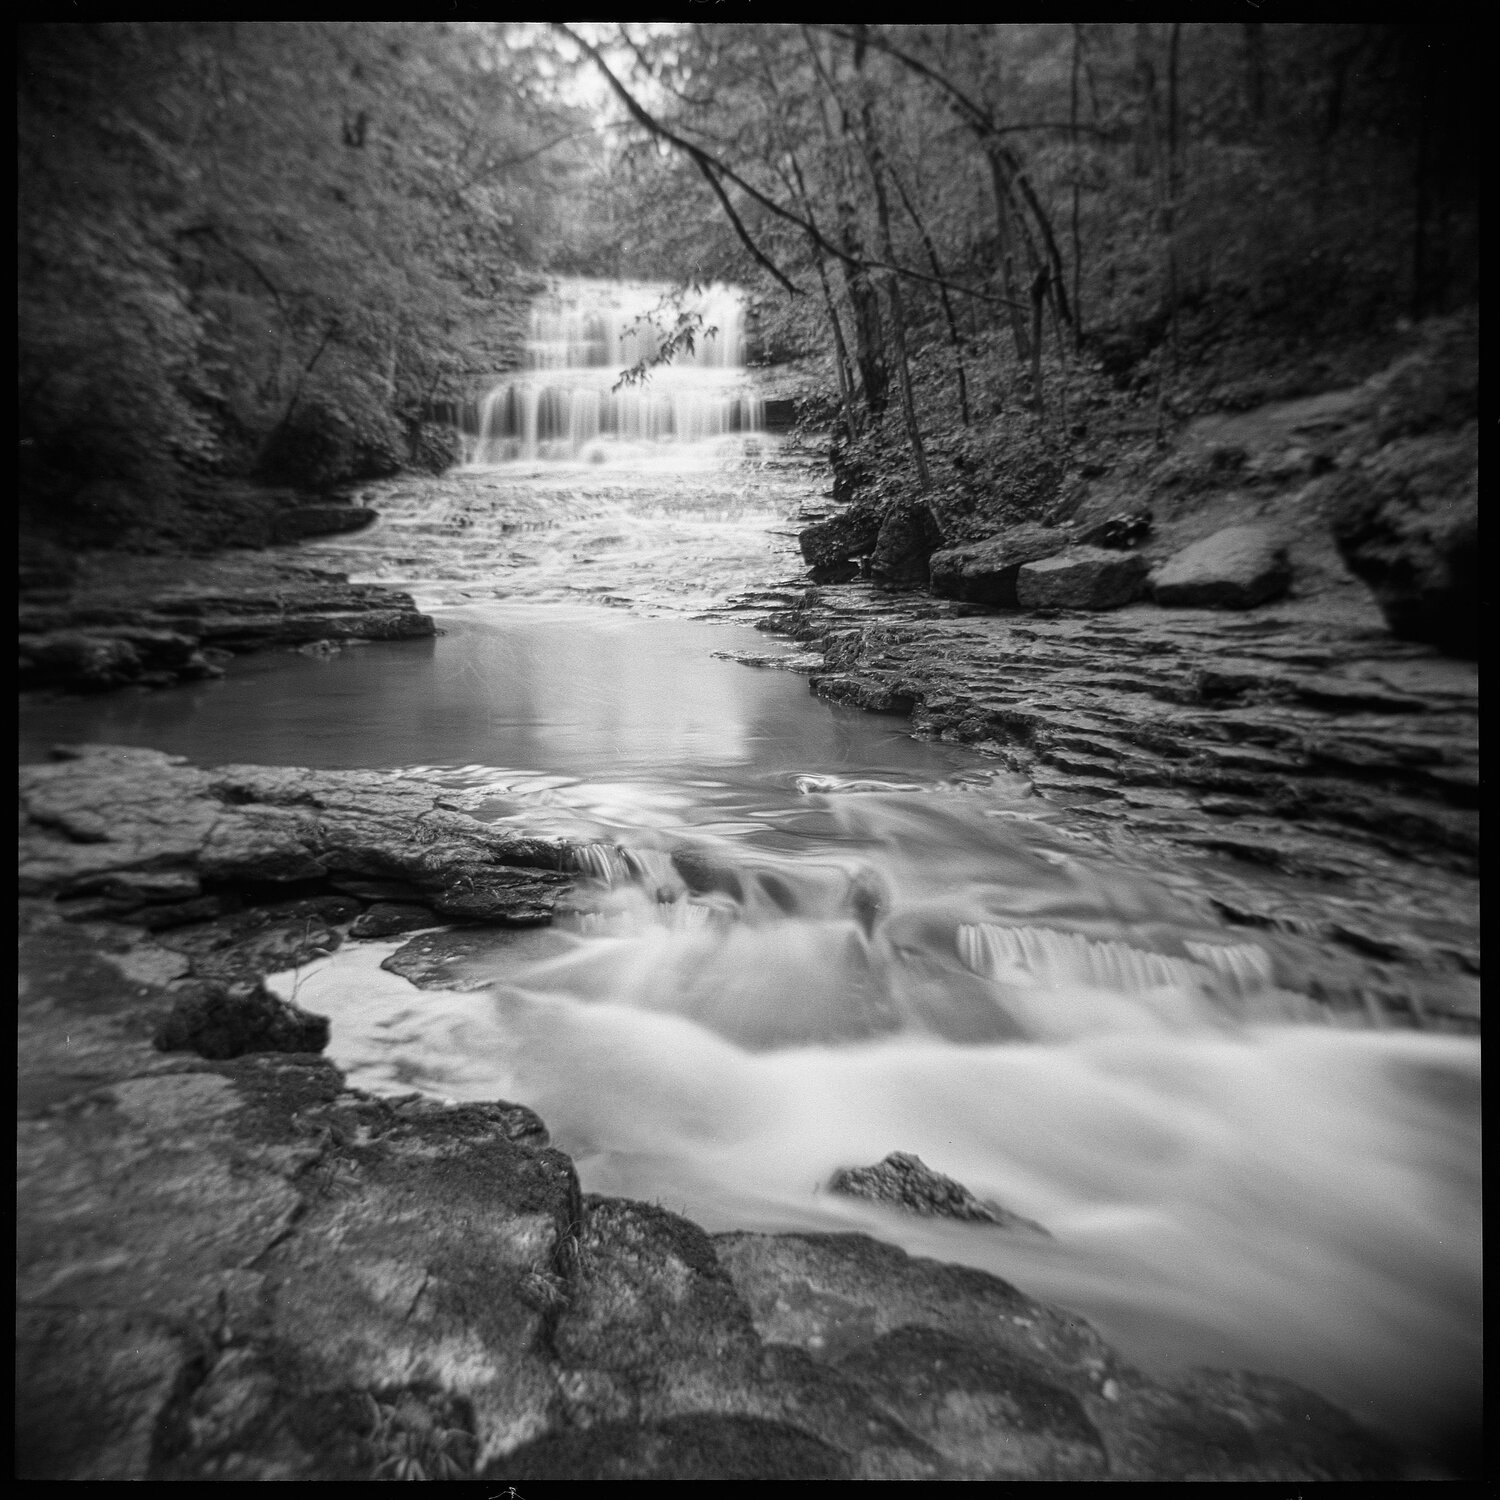
\includegraphics[width=90mm]{img/49929821132_d892aef245_k.jpeg}
    \caption{Fallsville Falls - Holga 120N. The leading lines of the water lead the viewer up to the main falls. The only consideration here is that this was shot with a Holga. That means generally only the center is sharp, so the main falls aren’t exactly sharp. I still like it though. To be honest most work done with a Holga is very subjective. Its a love it or hate it thing.}
\end{figure}

\section*{RULE OF THIRDS (ugh!)}
Yes, this one still has its place in square format. The difference  is that if you break the square frame down into thirds, you theoretically end up with 9 squares in grid, so that if you strictly follow this rule, some subjects, if they are large, *may* appear too close to the edge of the frame. This is one of those old rules that still, when it works, it just works.   

\begin{figure}[ht!]
    \centering
    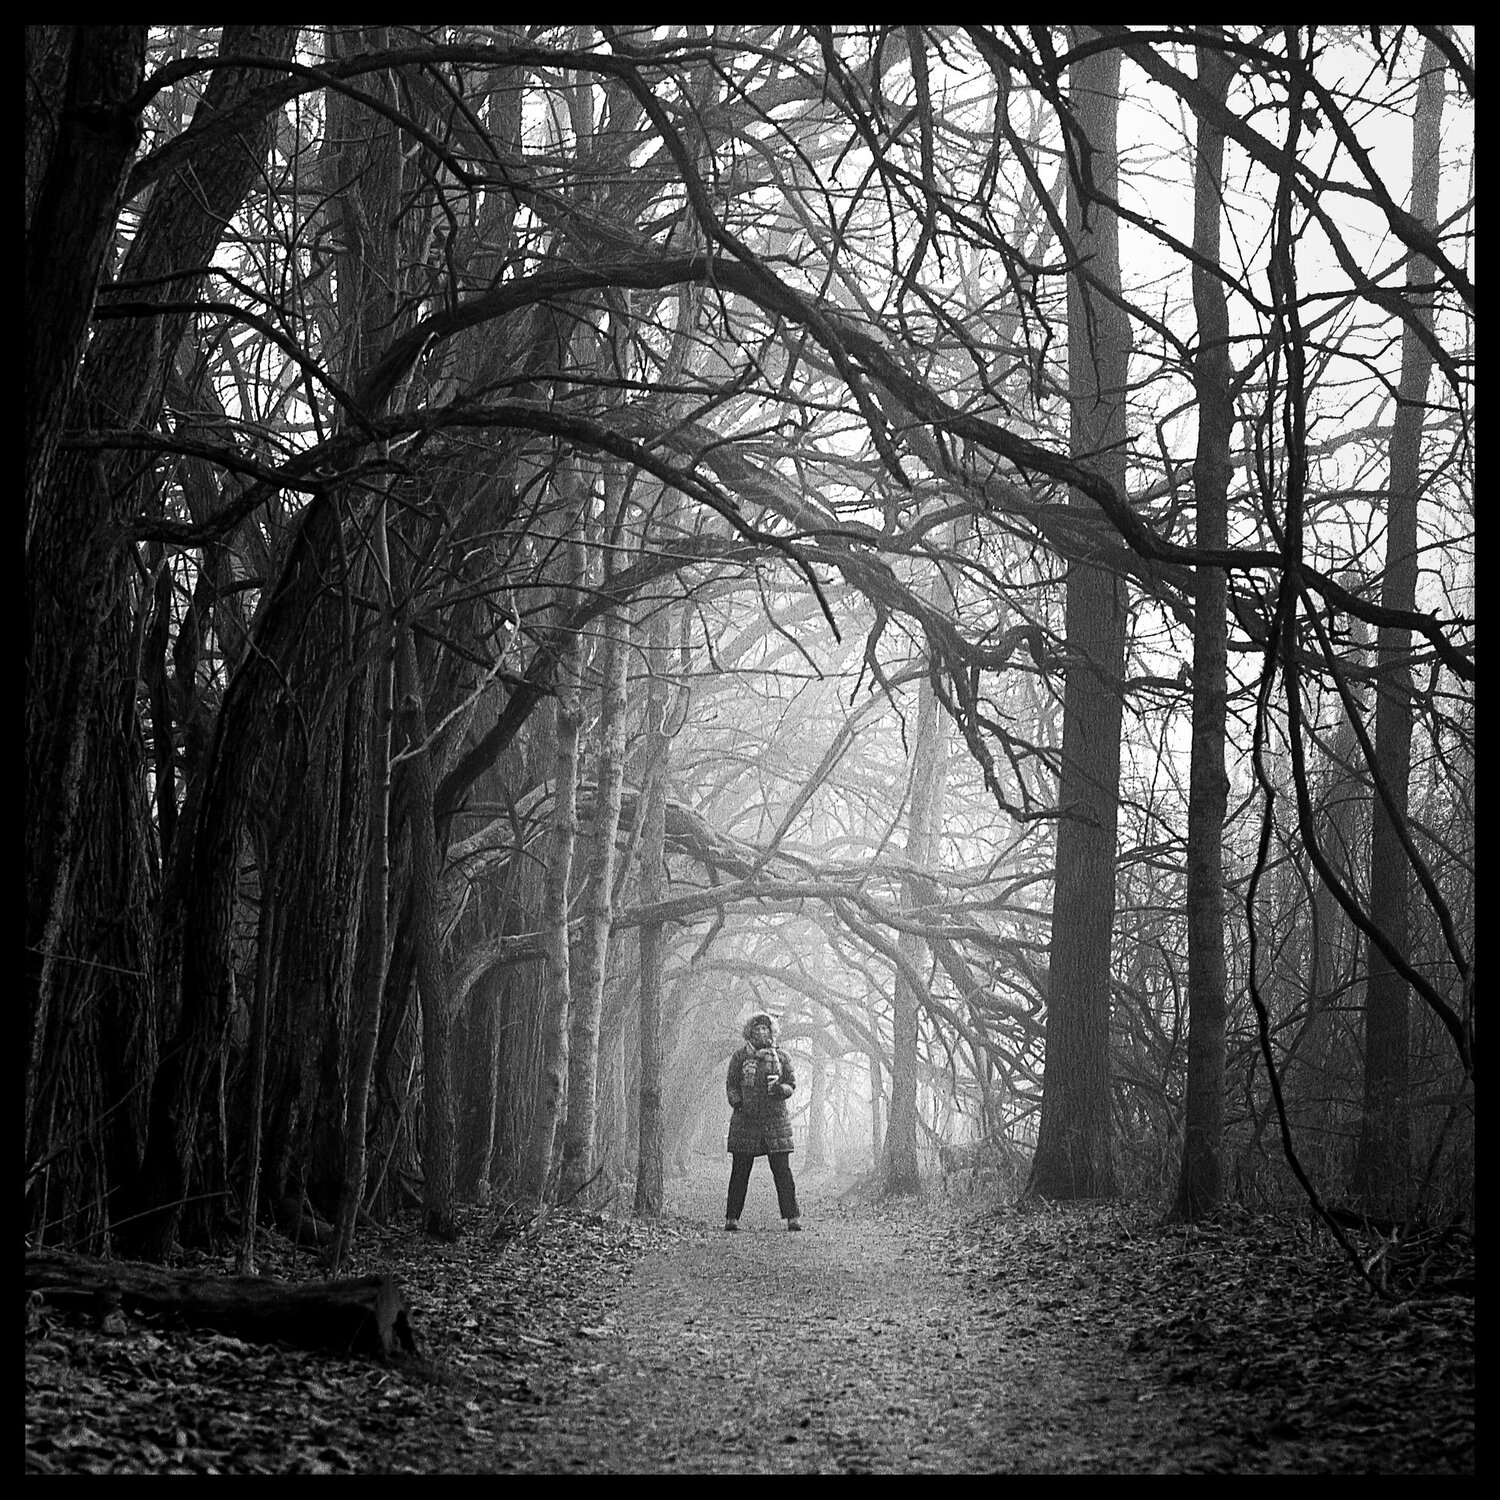
\includegraphics[width=90mm]{img/49286859422_ca0d380757_k.jpeg}
    \caption{Morning Coffee in Sugarcreek - Hasselblad 500c. I placed Renee at the bottom third of the image here. The distance and placement of subject help convey “smallness” in the natural setting. The fog that morning was a bonus.}
\end{figure}


\begin{figure}[ht!]
    \centering
    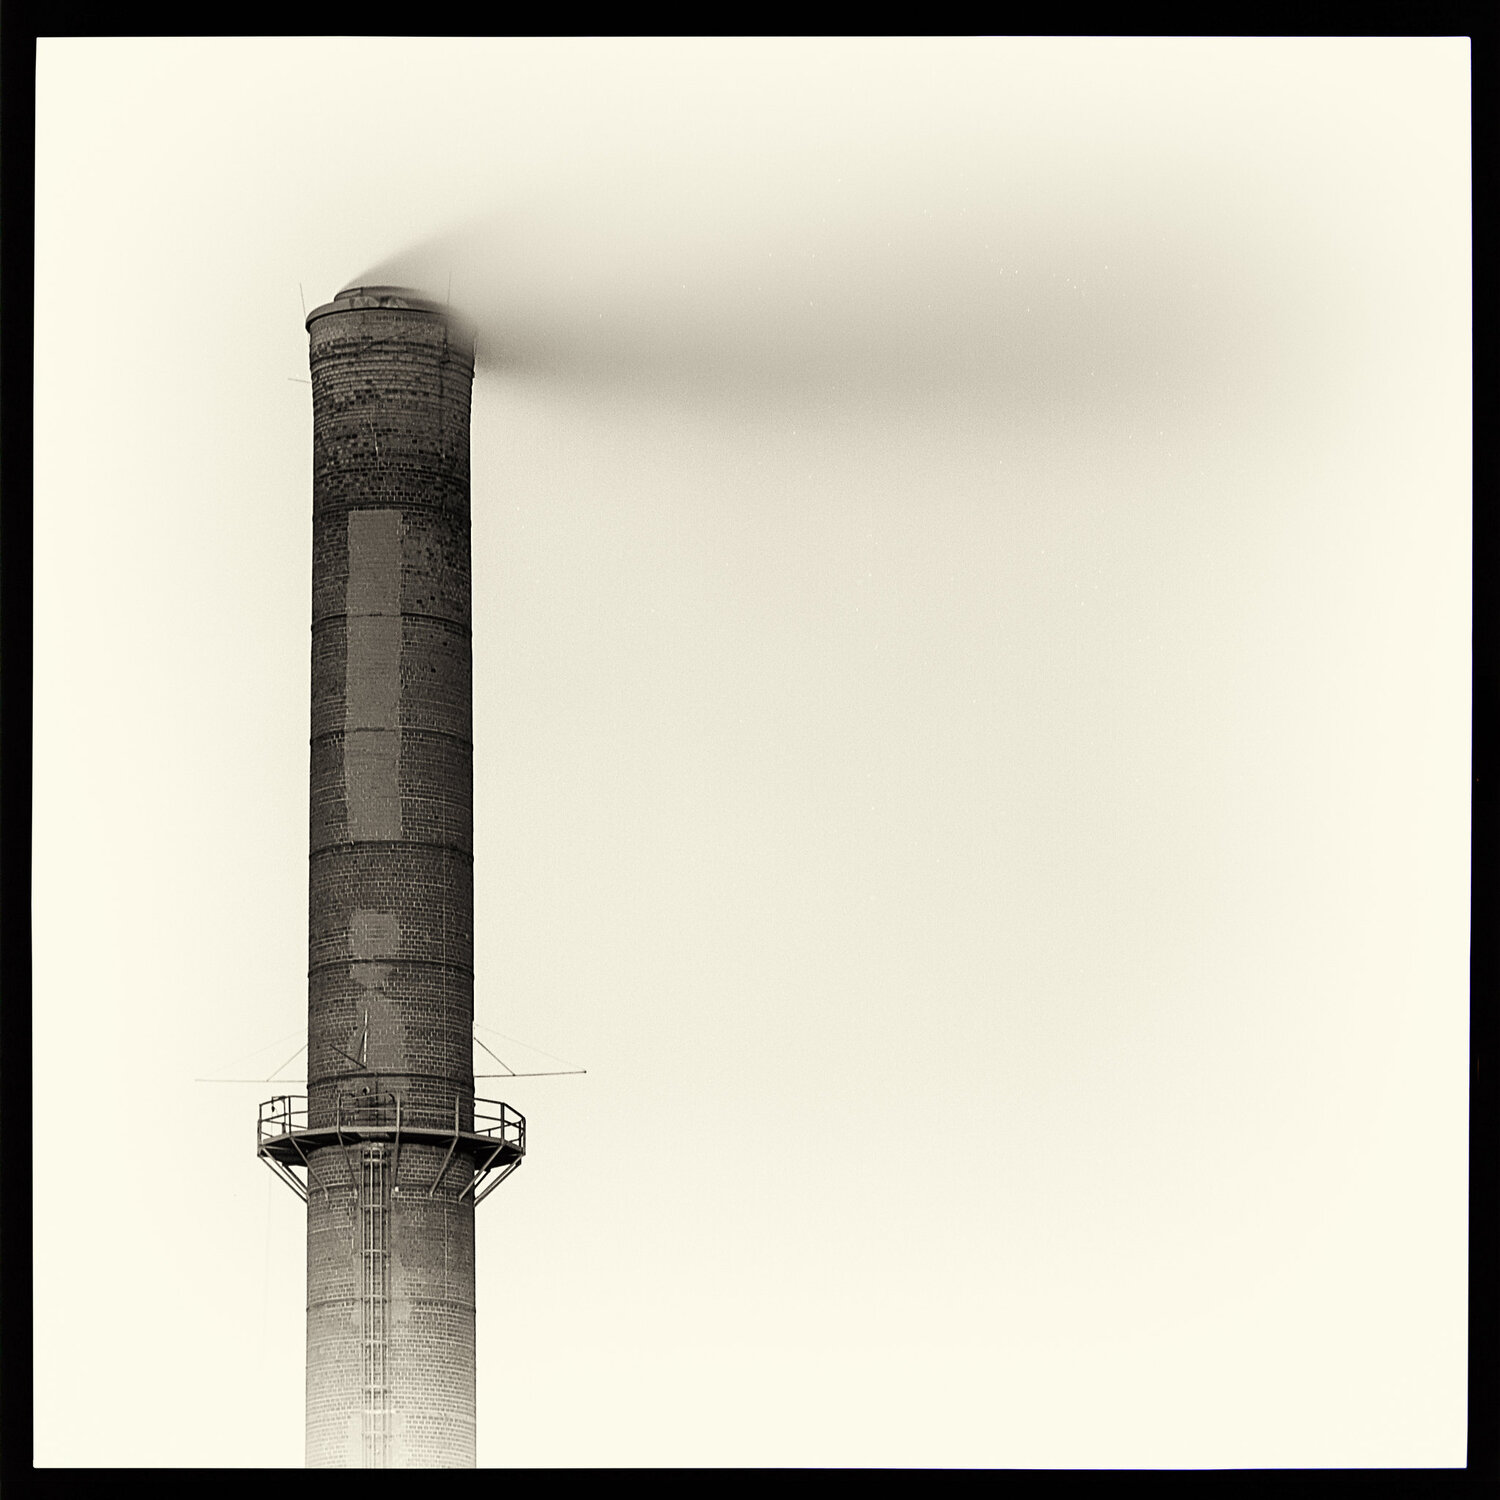
\includegraphics[width=90mm]{img/39124998042_470b8027ca_k.jpeg}
    \caption{Middletown Smokestack - Bronica S2A., long exposure. I shot this smokestack with several different compositions, but the one that worked best was this one - it allowed the smoke to not be cut off on the right. Even though the stack is really just slightly left of the thirds line, its close-enough.}
\end{figure}


\section*{LASTLY – BREAK ALL OF THE RULES} 
with the popularity of Instagram, there are a LOT of square images out there with all sorts of rule-breaking going on, and, surprisingly, I’ve found myself “liking” images that there is no way I thought I’d like if someone explained them to me. But visually they are just arresting and interesting. Below are a few of my own shots that do some rule-breaking.

\begin{figure}[ht!]
    \centering
    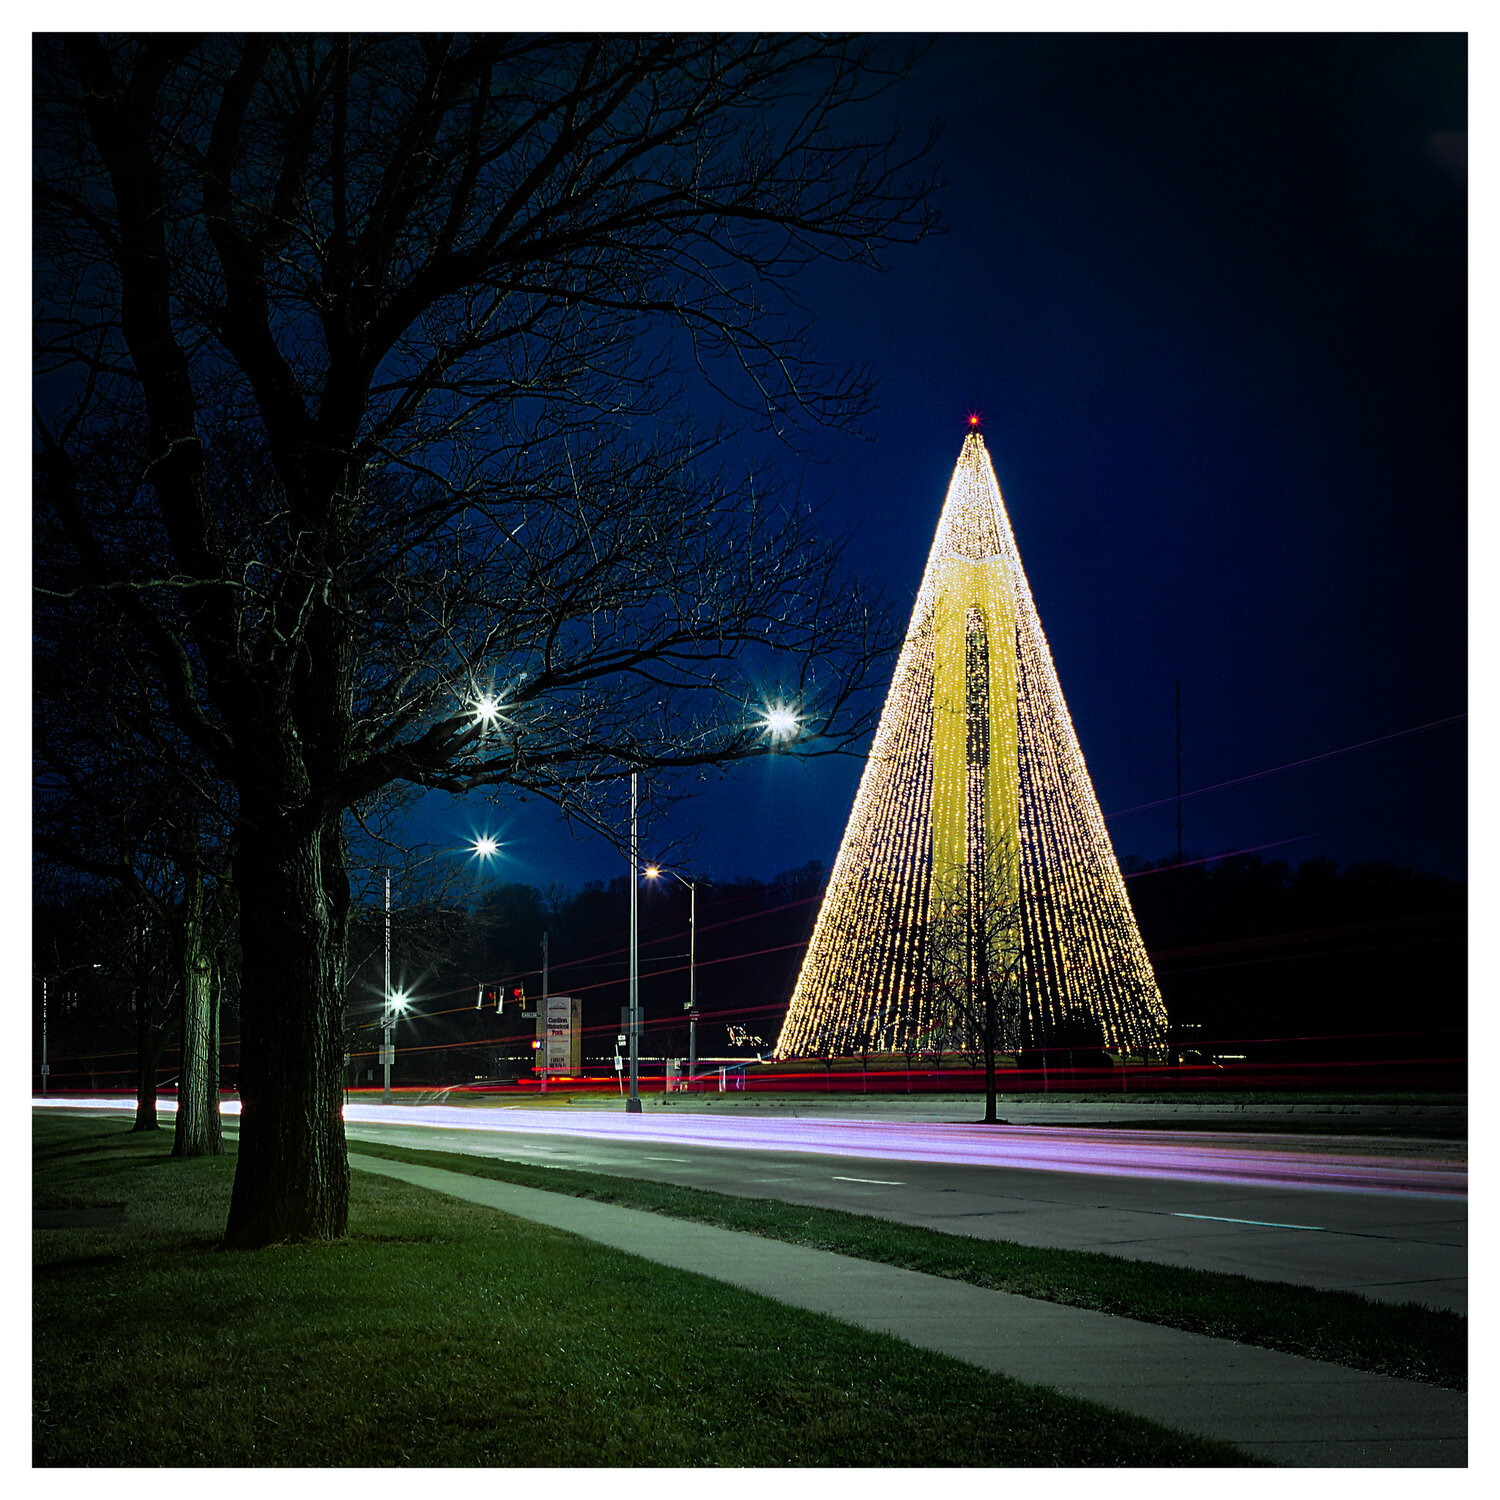
\includegraphics[width=90mm]{img/49224779302_9fe121cc9a_k.jpeg}
    \caption{Carillon Bell Tower - Hasselblad 500c on Ektar film. This one doesn’t really conform to the rules perfectly. The leading line of the cars going by doesn’t lead to anything, and the tower with the Christmas lights on it isn’t exactly on the thirds line. And the tree is cut off on the left. I could go on about the “fails” on this one but I still like it for some reason. Maybe because it makes me think of a Pink Floyd album cover.}
\end{figure}

\begin{figure}[ht!]
    \centering
    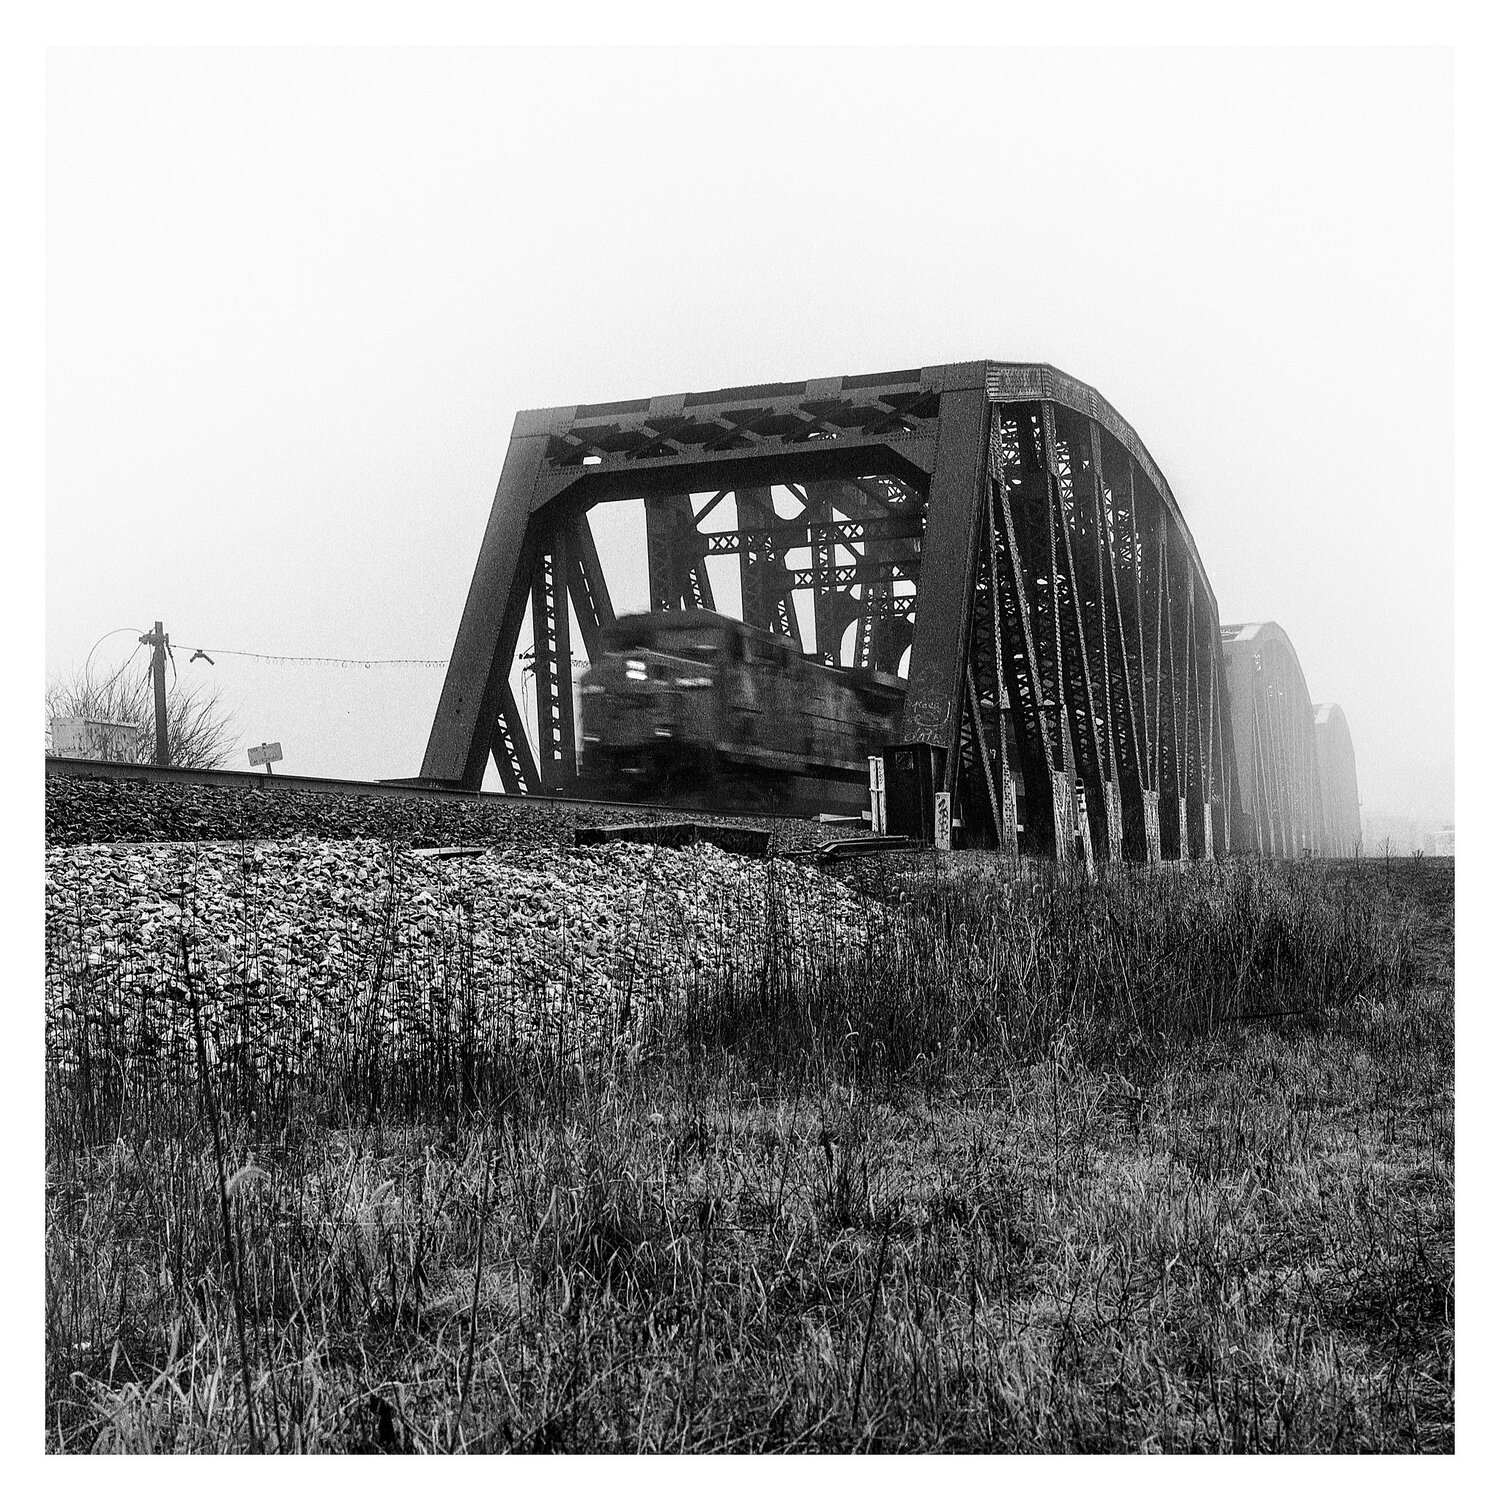
\includegraphics[width=90mm]{img/40177654042_f149a233ca_k.jpeg}
    \caption{Dayton Train - Hasselblad 500c on Trix-400 film. The subject isn’t exactly in the middle, there is probably too much foreground, and there’s motion blur on the train. What do I like about it? The fog in the background and the motion blur of the train. This may have worked better in a horizontal 4x5 ratio in retrospect. I’m not going top crop it though.}
\end{figure}

\begin{figure}[ht!]
    \centering
    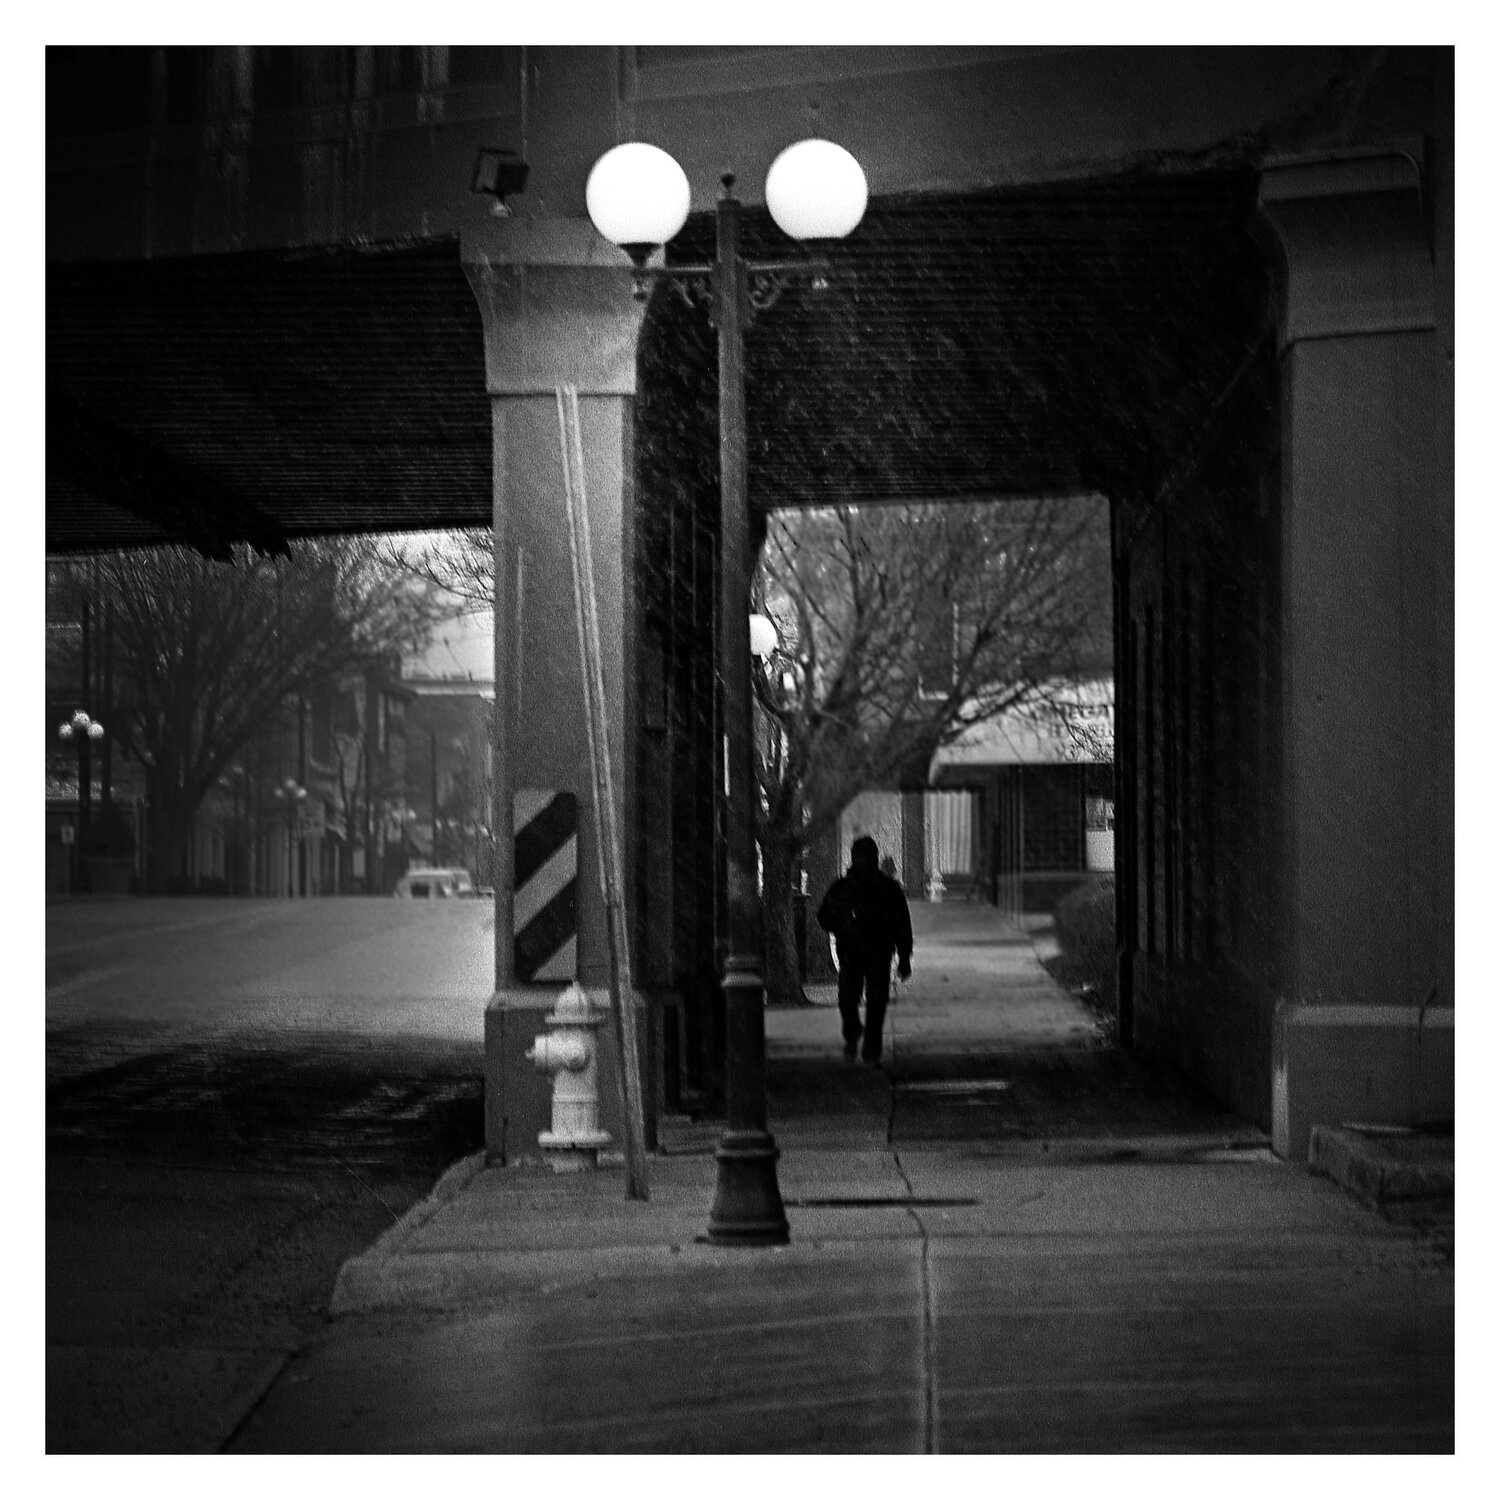
\includegraphics[width=90mm]{img/39970026082_4798ac7249_k.jpeg}
    \caption{Oregon District - Bronica S2A on Tri-X 400 film. This one breaks so many rules I’m not going to even start. What works for me? The weather/atmosphere, the lights on the lampost illuminating the freezing rain that’s falling, and the dark figure walking in the tunnel with the lit cigarette.}
\end{figure}

Hopefully this gives you a little insight into composing with a square format camera. Once you’ve done it for awhile you start seeing compositions while you are walking around that would look good in square. And maybe it just might be hard for you to go back to that boring old rectangle once again.  



\end{document}